\begin{translation}
\label{cha:translation}

\title{基于生成式预训练Transformer(GPT)和相对注意力的从头药物设计}
\maketitle

\tableofcontents
\author{Suhail Haroon *, Hafsath C.A., Jereesh A.S. *}

\begin{abstract}

  从头药物设计是指利用计算方法从头开始设计新药物分子的过程。与主要关注修改现有分子的其他计算方法相比,从头开始设计可以探索新的化学空间,并有可能发现具有增强特性的新型分子。在这项研究中,我们提出了一个利用生成预训练Transformer(GPT)架构和对从头药物设计的相对关注的模型。 GPT 是一种语言模型,利用 Transformer 架构来预测给定序列中的下一个单词或标记。使用 SMILES 符号表示分子使得在从头药物设计中使用下一个标记预测技术成为可能。 GPT 使用注意力机制来捕获序列中不同标记之间的依赖和关联,使得模型在处理输入时关注最重要的信息。

  相对注意力是注意力机制的一种变体,它使得模型捕获输入序列中标记之间的相对距离和关系。在标准注意力机制中,位置信息通常使用固定位置嵌入进行编码,而在相对注意力中,通过结合相对位置编码,我们可以在注意力计算期间动态提供位置信息,使模型能够快速学习新的未见标记的语法。

  相对注意力使 GPT 模型能够更好地理解序列中标记的相对位置,这在处理有限的数据集大小或生成特定目标药物时特别有用。本研究提出的模型在基准数据集上进行了训练,与其他生成模型比较了性能,结果表明,相对注意力和迁移学习可以使 GPT 模型在从头药物设计的背景下生成具有更高有效性、独特性和新颖性的分子。为了说明相对注意力的有效性,我们在三个特定目标数据集上使用迁移学习训练了该模型,并将性能与标准注意力进行了比较。
  \thusetup{
    keywords = {药物设计, 靶向药物, 屏蔽自注意力, 相对注意力, 从头药物设计, Transformer, 解码器, 生成式预训练模型}
  }
\end{abstract}


\section{简介}

药物设计和开发是制药公司和化学科学家的一个重要研究领域。药物开发是一个资源密集型过程,可能耗资 5 至 26 亿美元,耗时 10 至 20 年(Paul 等人,2010;Avorn,2015)。化学空间中的类药物化合物可能有 $10^{23}-10^{60}$ 之多 (Polishchuk 等人, 2013)。据估计,其中仅有 $10^8$ 个分子被合成(Kim 等人,2016),这表明很有可能存在更好的成药化合物,而更好地探索化学空间是非常必要的。通过临床前测试的五千种候选药物中,只有五种能够进入人体测试,并且经过人体测试的其中只有一种被批准投放市场(Mouchlis 等人,2021)。使用传统方法筛选无限化学空间具有挑战性且成本高昂,促使科学界将注意力转向基于人工智能的生成模型,这类模型可以提出潜在有价值的分子(Blaschke 等人,2020)。

基于机器学习的定量构效关系 (QSAR) 方法可作为虚拟筛选 (VS) 的关键过滤器(Bajusz 等人,2017)。这些方法可以有效、准确地评估理化和药理特性(Zheng 等人, 2017)。然而,这些方法通常依赖于现有的化学库来识别具有所需特性的分子。相比之下,从头药物设计通过从头开始生成具有理想药理和理化特性的新型分子来探索化学空间(Wang 等人,2022)。麻省理工学院 (MIT)《技术评论》将深度学习在药物发现中的应用评选为2020年十大突破性技术之一(Breakthrough,2020)。

多种架构,包括条件循环神经网络(RNN)、具有长短期记忆(LSTM)单元的 RNN(Hochreiter 和 Schmidhuber,1997 年)、变分自编码器(VAE)(Gomez-Bombarelli 等人,2018 年;Blaschke 等人,2018 年)和生成对抗网络(GAN)已经证明了它们基于分子数据表示生成分子的能力(Li 等人,2018; Weininger, 1988; Prykhodko 等人,2019; Kotsias 等人,2020a ;Pathak 等人,2020)。这些模型学习概率分布并通过对学习的分布进行采样来生成新分子。简化分子输入行输入系统(SMILES)(Weininger,1988)将分子表示为字符序列,促进了现代自然语言处理(NLP)技术在药物设计中的应用(Pathak 等人,2020)。

Transformer(Vaswani 等人,2017)是一种神经网络架构,近年来彻底改变了 NLP 领域。 Transformer 背后的核心思想是自注意力机制,它允许模型在生成输出序列时了解输入序列不同部分的重要性。这种机制在捕获文本数据中的长期依赖性方面特别有效,并导致 NLP 模型性能的显着提高。 Transformer包括编码器和解码器模块。生成式预训练 Transformer 模型(GPT)(Radford 等人,2018)仅使用 Transformer 的解码器部分,已独立用于语言建模任务。 MolGPT(Bagal 等人,2021)使用 GPT 的架构进行分子生成。使用两个基准数据集 MOSES (Polykovskiy 等人,2020) 和 GuacaMol (Brown 等人,2019) 来训练和评估 MolGPT 的性能。该模型在预测具有所需特性的新型化合物方面显示出显著的效果。

\section{文献综述}

药物设计已成为制药领域日益重要的研究领域。近年来,人们对将深度学习的前沿进展应用于药物设计的兴趣激增。最初,NLP 中使用的技术(Segler 等人,2018 年;Voss,2015 年)适用于类药物分子的预测。使用 SMILES 字符串训练的 RNN 可以生成比原始训练数据集大得多的化学空间。强化学习 (RL) 在药物设计中广受欢迎,可用于生成具有所需特性的分子。强化学习使用一个代理与环境交互,并从反馈中以奖惩的形式进行学习。在药物设计中,环境是化学空间,而代理是一个生成分子以最大化特定的奖励函数的生成模型。奖励函数可以基于药物相似性、生物活性或合成可行性等特性。 REINVENT 方法将 RNN 与强化学习相结合,生成具有所需特性的结构(Olivecrona 等人,2017)。随后,VAE 也被应用于药物设计,利用编码器将分子转换为潜在向量表示,并利用解码器从潜在表示重建原始分子。通过操纵和解码内部潜在表示,我们可以创建新的化学空间。随机 SMILES(Bjerrum,2017)生成的潜在表示具有增强的质量。

GAN(Goodfellow 等人,2020)是一种人工神经网络,由两部分组成:生成器和判别器,它们相互竞争。 GAN 通过生成模仿训练数据集的新数据样本,在图像和视频合成、文本生成等各个领域显示出了有前景的结果(Karras 等人,2017)。生成器生成新的数据样本,而鉴别器区分真实数据和生成数据。训练持续进行,直到鉴别器无法区分真实数据和生成数据。 GAN 在分子生成中的第一个应用是 ORGAN (Guimaraes 等人,2017),其改进版本 ORGANIC (Sanchez-Langeling 等人,2017) 是专门为逆向分子设计而设计的。 RANC(Putin 等人,2018a)和 ATNC(Putin 等人,2018b)将 GAN 与 RL 相结合,利用了一种更加先进的 RNN 架构——差分神经计算机(DNC)(Graves 等人,2016),而非中央 RNN。基于 DNC 的架构可以处理更长的 SMILES 并生成更多样的分子。

LatentGAN(Prykhodko 等人,2019)引入了一种新颖的分子生成方法,它将自动编码器与 GAN 集成在一起。该模型将一个 SMILES 异质编码器训练出的自动编码器(Kotsias 等人,2020b)来获取每个 SMILES 的 n 维向量。因此,该模型可以使用潜在表示,而无需处理 SMILES 语法。预训练异质编码器的解码器部分(Bjerrum 等人,2018)将生成的 n 维向量转换为分子结构。贝叶斯优化(Gómez-Bombarelli 等人,2018;Mehta 等人,2021)等方法也已用于生成具有所需特性的分子。 Mol-Cycle GAN 利用 CycleGAN(Maziarka 等人,2020;Zhu 等人,2017)的损失来生成具有所需特性的分子。Tao Song 等人提出了 DNMG,一种利用配体的 3D 信息进行从头药物设计的深度分子生成模型(Song 等人,2023)。他们用一个基于 Wasserstein GAN 的网络根据 3D 网格空间信息和配体的原子物理化学性质生成分子的表示,然后使用字幕网络将生成的表示解析为 SMILES 字符串。 DNMG 能够生成具有更好结合能力的有效新型药物样配体,并已用于 MK14、FNTA 和 CDK2 三个靶点的抑制剂开发。

MolGPT(Bagal 等人,2021)使用 Transformer(Vaswani 等人,2017)进行从头药物设计。Transformer模型由编码器和解码器模块组成。 GPT 指的是在语言建模任务中独立运行的 Transformer 解码器模块,(Radford 等人,2018)。 GPT 模型已有效应用于各种 NLP 任务中(Radford 等人,2019)。 MolGPT 是第一个基于 GPT 架构的分子生成模型。它使用 GPT 架构和自注意力机制来预测 SMILES token序列。它使用 SMILES 标记器,利用正则表达式从 SMILES 字符串中提取相关token,这些token是根据应用于所有先前生成的token的注意力来预测的。该模型能够生成具有所需特性的分子。

生物靶标的蛋白质信息可用于生成具有良好对接分数的药物。 Wang 等人(2023)提出的PETrans 利用目标蛋白信息来生成目标特异性药物。他们使用 GPT 提取分子的上下文特征。为了提取目标蛋白的氨基酸信息和理化特性,三种不同的蛋白质编码技术被采用,即联合三联体(CT)、伪氨基酸组成(pseAAC)和自相关描述符(AD)。首先通过蛋白质编码方法将蛋白质序列转化为512维向量,然后再结合蛋白质编码和分子序列信息促进分子生成。 Chen 等人(2023)提出的 Deep Target使用目标蛋白的氨基酸序列进行药物发现。它具有三个模块,即分子生成(MG)、结构特征推理(SFI)和氨基酸序列嵌入(AASE)。 AASE模块用于生成目标蛋白氨基酸序列的嵌入,SFI模块推导了合成分子的潜在结构特征,而MG模块则用于构建最终分子。

相对注意力(Shaw 等人,2018)是 Transformer 模型中引入的一种自注意力机制,用于提高需要捕获序列中标记相对位置的任务的性能。在传统的自注意力中,模型根据每对标记在序列中的绝对位置来计算它们之间的注意力分数。然而,在许多任务中,标记的相对位置比其绝对位置更重要。本文展示了相对注意力在药物设计中的运用。 MolGPT 被用作 Transformer 解码器模型,成为应用相对注意力的对象。所得模型的性能与具有标准注意力机制的原始 MolGPT 模型进行了比较。

\section{材料和方法}

\subsection{数据集}

MOSES 和 GuacaMol 数据集被用于训练和评估模型。 MOSES 数据集包含来自 Zinc 数据集的 190 万个干净的先导样分子(Irwin 和 Brian,2005)。 GuacaMol 包含 160 万个分子,它们是 ChEMBL 24(Gaulton 等人,2017)数据库的子集。为了将工作扩展到目标特定数据集,我们从 ExCAPE-DB 下载了 HTR1A、S1PR1 和 EGFR (Sun 等人,2017)。为了提取分子特性,我们使用了骨架 RDkit 工具包(Landrum,2018)。该模型经过训练可以无条件或有条件地生成分子。在无条件生成中,要求模型生成具有与数据集中的药物相似的性质的类药物分子;在条件生成中,要求模型生成具有特定用户定义属性(如 logP、QED 等)值的类药物分子。在条件生成过程中,所需的条件将作为模型的输入。

\subsection{具体方法}

MolGPT 对各个标记采用位置值嵌入来维护输入序列的顺序。分段标记用于区分条件标记和 SMILES 标记,帮助模型区分输入条件和 SMILES 标记。每个分子的 SMILES 标记、位置标记和片段标记通过专用的可训练嵌入层单独转换为 256 维向量。然后将生成的 SMILES 标记嵌入、位置嵌入和段标记嵌入组合起来,为 SMILES 字符串的每个标记生成一个 256 维向量。随后将该向量作为输入提供给模型。

MolGPT 采用掩蔽自注意力机制来防止模型在训练过程中预测未来的标记。在掩蔽自注意力中,输入序列首先被转换为三种类型的向量:键向量、值向量和查询向量。查询向量表示序列中的当前元素,而键和值向量表示序列中的其他元素。

注意力定义为:

\begin{equation}
  Attention(Q,K,V)=softmax({QK^T}/ {\sqrt{d_k}})V
\end{equation}

K、Q 和 V 分别对应于键、查询和值向量,查询和关键向量维度表示为$d_k$,T表示矩阵的转置。

序列中的每个位置使用位置嵌入分配一个固定的嵌入向量。然而,这种方法无法捕获token的相对位置,从而无法更好地理解序列的上下文。

Shaw 等人(2018)引入了具有相对位置表示的自注意力机制,这是一种有效结合序列元素之间的相对位置或距离表示的技术。使用两个数据集在 WMT 2014 机器翻译任务上评估了该方法的有效性:WMT 2014 英语-德语数据集(包含约 450 万个句子对)和 WMT 2014 英语-法语数据集(包含约 3600 万个句子对)。结果表明,对于英德翻译任务,相对位置方法将基本配置和大配置的性能分别提高了 0.3 和 1.3 BLEU。对于英法翻译任务,相对位置方法使基本配置和大型配置的性能分别提高了 0.5 和 0.3 BLEU。

自注意力子层使用注意力头来生成输入序列的多种表示。每个头的结果通过串联进行组合,并应用具有学习参数的线性变换来产生子层输出。

对于一个长度为$n$的输入序列$\boldsymbol{x} = \left( x_1, \ldots, x_n \right), x_i \in \mathbb{R}^{d_x}$,我们计算一个新序列$\boldsymbol{z} = \left( z_1, \ldots, z_n \right)$。每个输出元素$z_i$为线性变换的输入元素的加权和:

\begin{equation}
  z_i = \sum_{j=1}^n \alpha_{ij} \left( x_jW^{v} \right)
\end{equation}

其中权重系数$\alpha_{ij}$使用 softmax 函数计算:

\begin{equation}
  \alpha_{ij} = \frac{\exp \left( e_{ij} \right)}{\sum_{k=1}^n \exp \left( e_{ik} \right)}
\end{equation}

$e_{ij}$使用比较两个输入元素的兼容性函数计算:

\begin{equation}
  e_{ij} = \frac{\left( x_iW^{Q} \right) \left( x_jW^{K} \right)^T}{\sqrt{d_z}}
\end{equation}

$W^Q, W^K, W^V \in \mathbb{R}^{d_x  \times d_z}$是参数矩阵。

我们使用键和值向模型提供相对位置信息(Tae,2023)。等式(2)和(4)被修改以合并相对位置信息。首先,相对位置信息作为键的附加组件提供给模型:

\begin{equation}
  e_{ij} = \frac{\left( x_iW^{Q} \right) \left( x_jW^{K} + a_{ij}^K \right)^T}{\sqrt{d_z}}
\end{equation}

Softmax 函数保持不变。

\begin{equation}
  \alpha_{ij} = \frac{\exp \left( e_{ij} \right)}{\sum_{k=1}^n \exp \left( e_{ik} \right)}
\end{equation}

随后,相对位置信息作为值矩阵的附加组件提供给模型:

\begin{equation}
  z_i = \sum_{j=1}^n \alpha_{ij} \left( x_jW^{v} + a_{ij}^V \right)
\end{equation}

“z”表示自注意力机制的输出。然后,该输出通过前馈神经网络,将“z”的表示形式转换为适合预测下一个标记的格式。前馈网络的变换输出随后被转发到投影层,该投影层将修改后的表示映射会回原来的词汇表大小,然后在投影层的输出应用一个 softmax 激活函数。 Softmax 函数对词汇表中所有可能标记的分数进行归一化,从而生成词汇表上的概率分布。此分布中的每个元素表示相应标记作为下一个预测标记的可能性。 softmax 输出中概率最高的token被视为预测的下一个token。

Peter Shaw 引入的附加相对位置编码矩阵的计算需要 $O(L^2D)$ 内存,其中$L$是序列的长度,$D$ 表示隐藏状态维度。Huang 等人(2018)提出了一种计算相对位置编码的新方法,该方法需要 $O(LD)$ 内存。例如,对于 2048 的序列长度和 512 的隐藏状态大小,每层的内存使用量从 8.5GB 减少到 4.2 MB(每个头从 1.1GB 减少到 0.52 MB)。内存使用量的减少使我们得以利用 GPU 在较长的序列上训练相对自注意力 Transformer。

根据 Huang 等人的说法。相对关注度计算如下:

\begin{equation}
  Relative\ Attention = softmax \left( \frac{QK^T + S_{rel}}{\sqrt{d_k}} \right)V
\end{equation}

Huang 等人没有关注与值项相对应的附加相对位置嵌入,而是仅关注了关键组件,并使用了一个额外的项 $S_{rel}$。

\begin{equation}
  S_{rel} = QR^T, R_{ij} = a_{ij}^K
\end{equation}

$\boldsymbol{R}$ 是相对位置嵌入的矩阵。Huang 等人引入了一种带有一组填充和矩阵运算操作的倾斜机制,无需显式计算 $\boldsymbol{R}$ 即可计算 $S_{rel}$。这消除了 $O(L^2d)$ 额外空间的巨大内存瓶颈。

\begin{figure}[H]
  \centering
  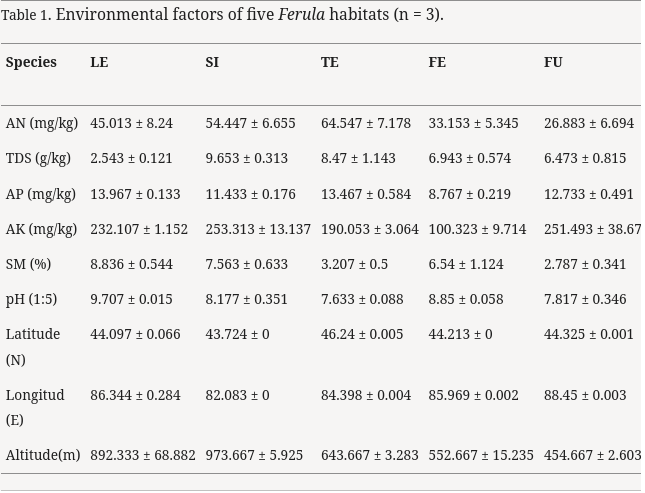
\includegraphics[width=\linewidth]{fig1.png}
  \caption{具有相对注意力结构的 MolGPT}
  \label{fig:1}
\end{figure}


所提出的模型如图 \ref{fig:1} 所示。模型利用 MolGPT 的架构,但用相对注意力取代了标准注意力。在 MolGPT 中,位置值嵌入被分配给每个token以维持序列顺序。然而,在新模型中,利用相对位置嵌入来进行相对注意力计算。这消除了直接将位置嵌入作为模型输入的需要,因为相对位置信息在注意力计算期间动态添加到键中。

该模型由八个堆叠的解码器块组成,每个解码器块包含一个屏蔽自注意力层和一个完全连接的神经网络。自注意力层产生大小为 256 的向量,然后将其馈送到全连接网络中。神经网络的隐藏层输出大小为 1024 的向量,然后将其传递到高斯误差线性单元 (GELU) 激活层。全连接神经网络的最后一层返回大小为 256 的向量,该向量用作下一个解码器块的输入。段标记用于区分条件标记和 SMILES 标记,帮助模型区分输入条件和 SMILES 标记。该模型采用屏蔽自注意力策略来防止模型在训练过程中预测未来的标记。

为了利用 SMILES 字符串标记之间的成对相对位置信息,MolGPT 中应用了相对注意方法。使用 MOSES 和 GuacaMol 数据集来训练和评估模型,并将其性能与标准注意力进行比较。然后将模型权重用于迁移学习,使其能够生成目标特定分子。

\section{结果和讨论}

使用相对注意力的 MolGPT 模型在四个数据集上分别进行训练:MOSES、GuacaMol、HTR1A 和 S1PR1。对 HTR1A 和 S1PR1 的子集进行随机采样,以评估较小数据集上的相对注意力表现。采样的 HTR1A 数据集由 3400 个 SMILES 组成,采样的 S1PR1 数据集由 796 个 SMILES 组成。采用迁移学习技术使用采样数据集生成特定目标的化合物。所提出的模型首先在 MOSES 数据集上进行训练,然后使用模型权重在采样的特定目标数据集上进行训练。该方法还扩展到包含 1380 个 SMILES 的 EGFR 数据集。

\subsection{考虑的属性}

以下属性用于评估模型在条件生成中的性能:

\begin{enumerate}[label=\alph*)]
  \item logP: \\在药物设计中,logP(也称为分配系数的对数)与药物的亲脂性或疏水性有关。它是平衡状态下分子在非极性溶剂(例如辛醇)中的浓度与其在极性溶剂(例如水)中的浓度之比。由于药物亲脂性的重要性,logP 是 Lipinski五规则的组成部分(Lipinski等人,2012)。logP 在确定药物在体内的吸收、分布、吸收和运输方面起着至关重要的作用。此外,logP 还指导药物的配方和剂量。它是 Lipinski 五规则指南的一个关键方面,用于预测新合成化合物用作药物的适用性。根据 Lipinski 五规则,为了获得最佳的口服和肠道吸收,药物的 logP 值理想应在 1.35 至 1.8 之间,且不应超过 5。
  \item 拓扑极性表面积 (TPSA):\\TPSA 值是通过使用基于分子拓扑的一组特定规则,总结分子中所有极性原子(例如氧和氮)及其附着的氢原子的贡献来计算的。结果值以平方埃 (Å$^2$) 表示。它类似于药物渗透细胞膜的程度。 TPSA 大于 140 Å$^2$ 的药物渗透细胞膜的能力较低。
  \item 综合辅助得分 (SAS):\\SAS 参数用于评估分子合成的难易程度(Ertl 和 Schuffenhauer,2009)。它的得分在 1(容易制备)和 10(极难制备)之间。分数计算为分子中所有片段贡献的总和除以该分子中片段的数量。
  \item 药物相似性定量估计 (QED):\\QED 用于在药物设计中估计分子的药物相似性(Bickerton等人,2012)。分数的值介于 0 和 1 之间。QED 分数为 1 表示该分子具有所需的药物样特性,而分数为 0 表示该分子不具有药物样特性。
\end{enumerate}

\subsection{使用的指标}

以下指标用于评估所提出模型的性能:


\begin{enumerate}[label=\alph*)]
  \item 有效性:指有效分子占生成分子总数的比例。使用 RDkit 检查生成分子的有效性。如果模型很好地学习了 SMILES 语法和原子的化合价,则模型生成的分子将具有更高的有效性。\\有效性=生成有效分子的总数/生成分子的总数
  \item 唯一性:它是指有效生成的分子中唯一的部分。如果模型的唯一性较低,则模型往往会重复生成相同的分子。\\唯一性=生成唯一有效分子的总数/生成有效分子的总数
  \item 新颖性:它是指模型相对于训练集生成的新颖的有效且独特的分子的比例。新颖性低表明模型过拟合。\\新颖性=生成新颖有效有效分子的总数/生成唯一有效分子的总数
\end{enumerate}
有效性、唯一性和新颖性的值落在 0 到 1 的范围内。

\subsection{结果分析}

MOSES 数据集包含来自锌数据集的 190 万个干净的类铅分子,具有理想的类药物特性。 GuacaMol 是 ChEMBL 24 数据库的子集,包含 160 万个分子。 MOSES 数据集具有前导样分子,因此导致分布表现出理想的类药物特性。 GuacaMol 数据集具有更广泛的属性值,因此比 MOSES 具有更大的分布。

\begin{figure}[H]
  \centering
  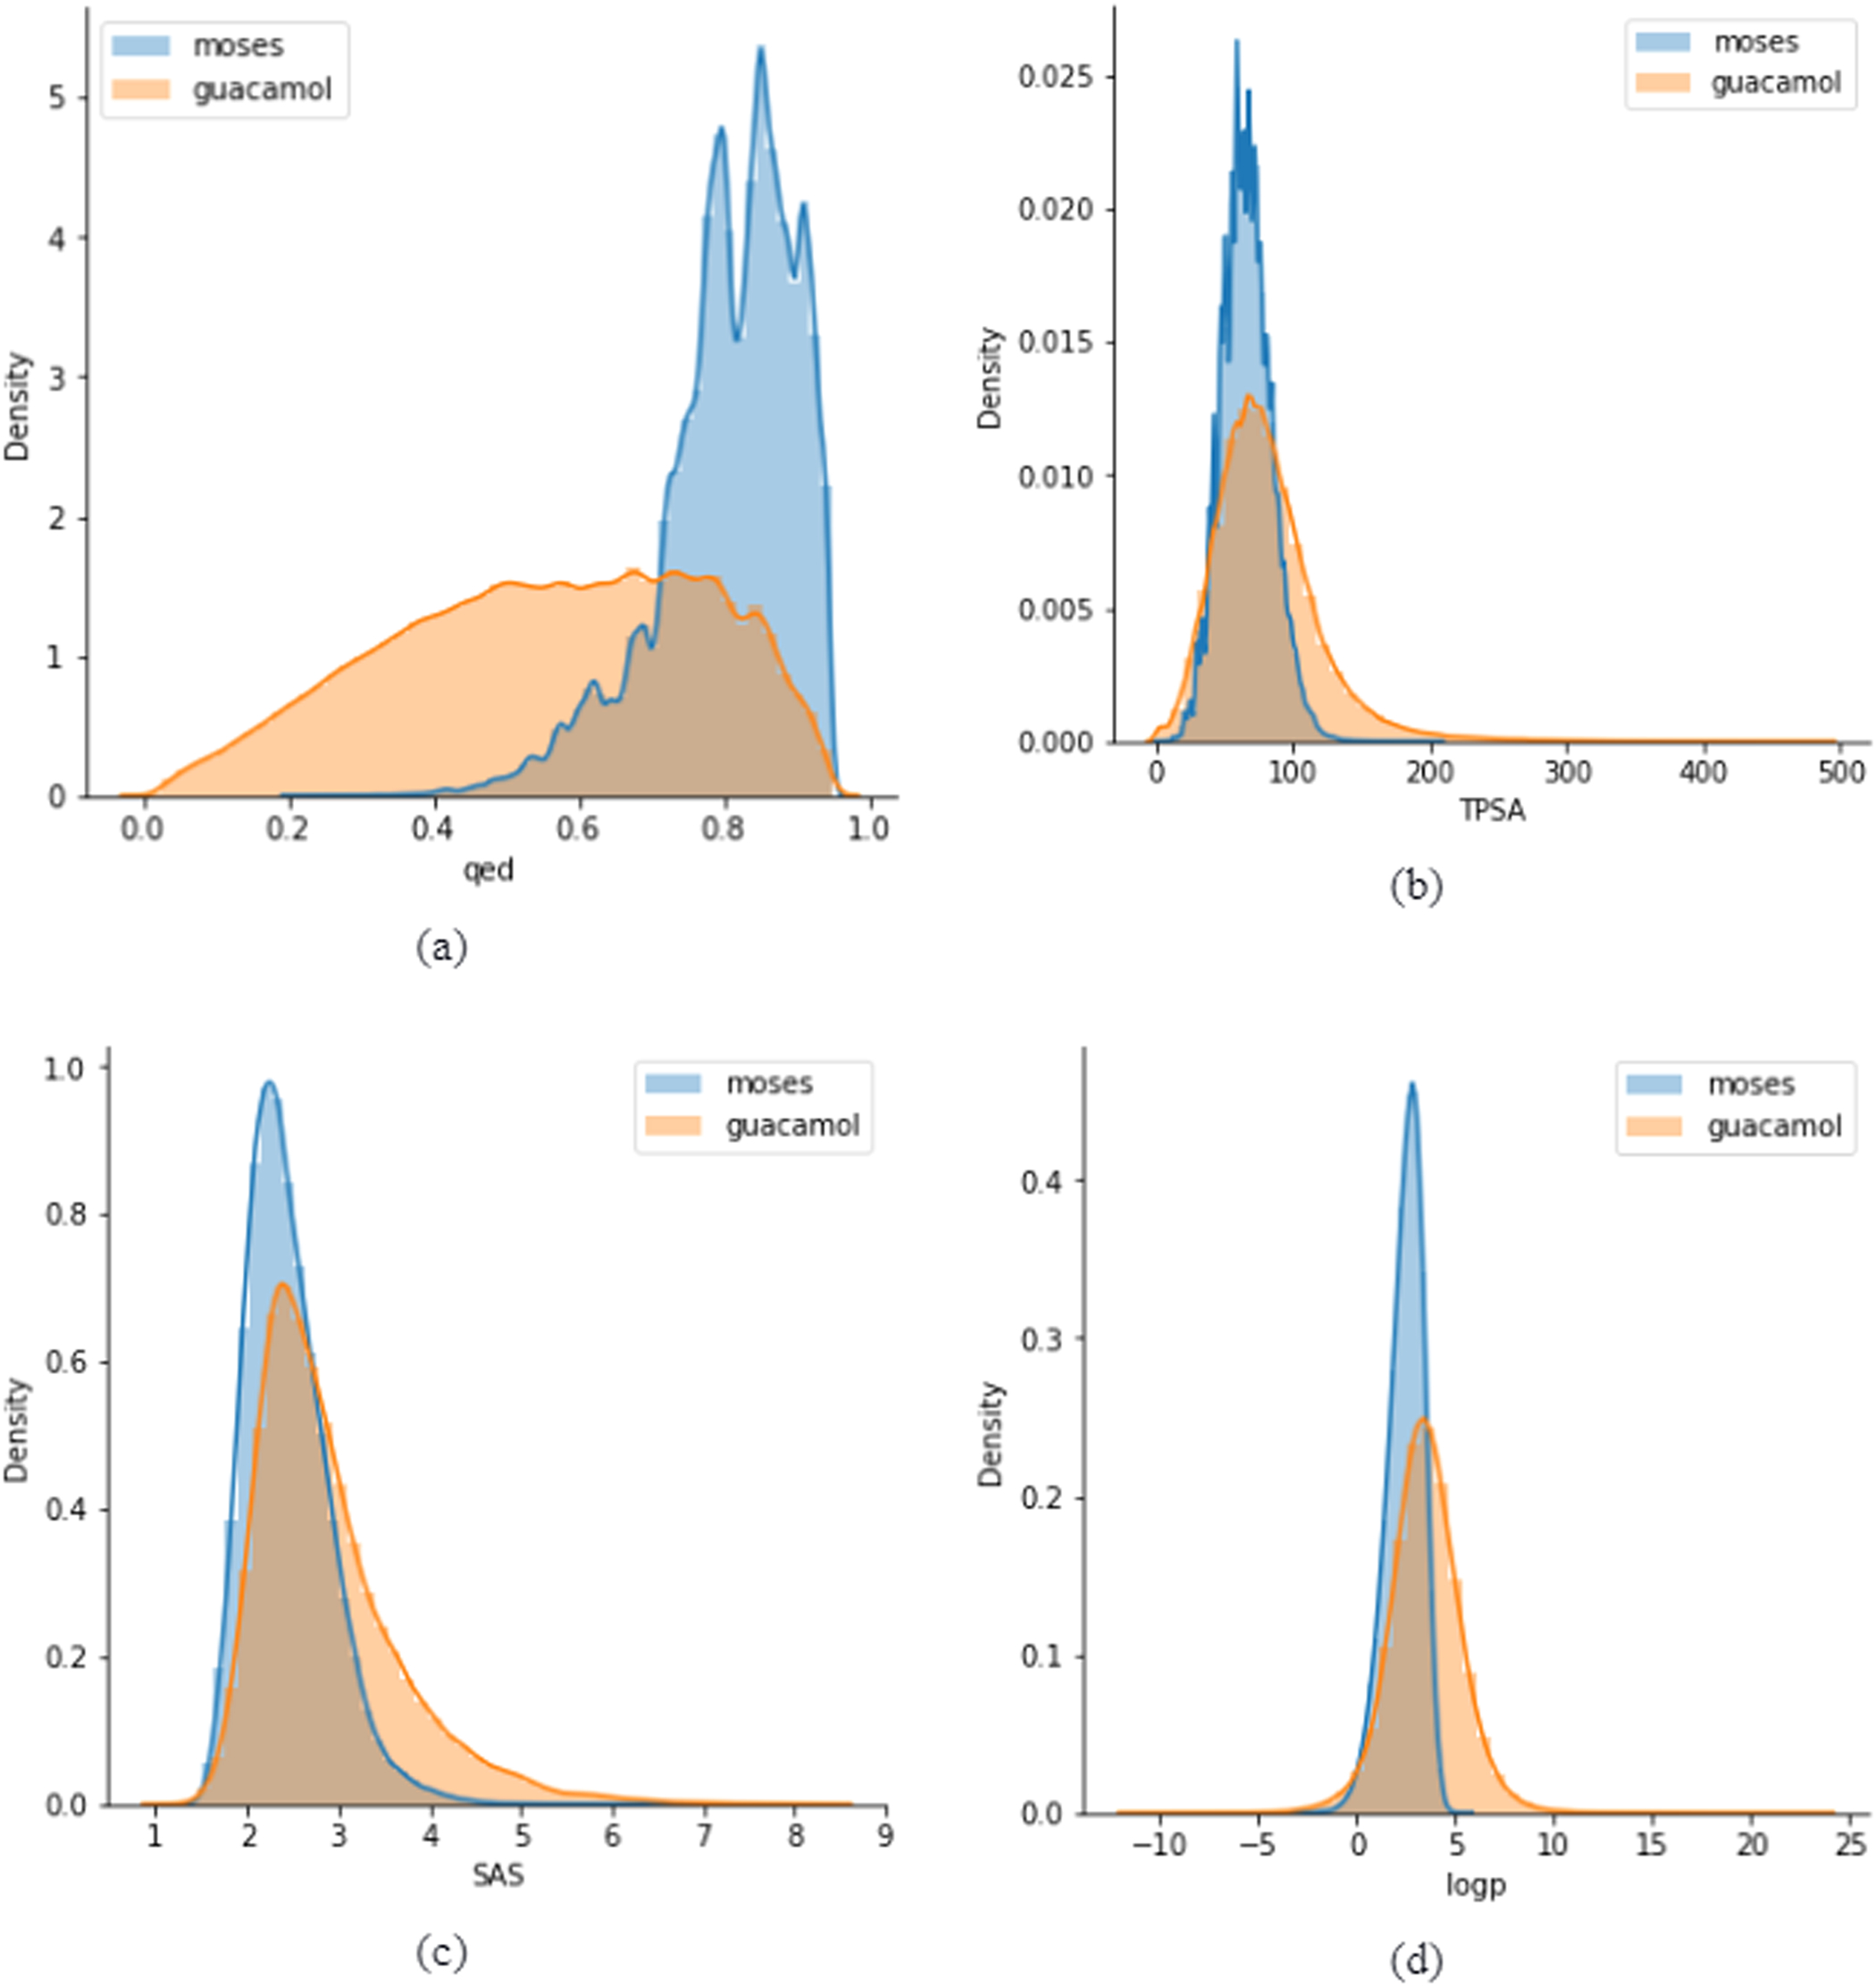
\includegraphics[width=\linewidth]{figures/2.png}
  \caption{MOSES 和 GuacaMole 中分子的性质(QED、TPSA、SAAS、aur logP)分布}
  \label{fig:2}
\end{figure}

MOSES 和 GuacaMol 数据集中药物不同属性的概率分布如图 \ref{fig:2} 所示。该分布提供了在数据集中遇到具有指定属性并落在特定范围内的药物的可能性的相对度量。 GuacaMol 数据集具有较大的属性值分布,因此用于测试模型生成具有不同属性值的分子的能力。

为了比较各种模型的性能,每个模型都被分配了预测 10,000 个分子的任务。随后,计算预测的 10,000 个分子集中有效、独特和新颖药物的百分比。

\begin{table}[H]
  \centering
  \caption{使用 MOSES 进行非条件生成训练的生成模型之间的比较}
  \label{tab:1}
  \begin{tabular}{llll}
    \hline 模型      & 有效性   & 唯一性@10 K & 新颖性   \\
    \hline AAE     & 0.937 & 0.997    & 0.793 \\
    VAE            & 0.977 & 0.998    & 0.695 \\
    CharRNN        & 0.975 & 0.999    & 0.842 \\
    LatentGAN      & 0.897 & 0.997    & 0.949 \\
    JT-VAE         & 1.0   & 0.999    & 0.914 \\
    MolGPT         & 0.994 & 1.0      & 0.797 \\
    使用相对注意力的MolGPT & 0.992 & 1.0      & 0.879 \\

    \hline
  \end{tabular}
\end{table}

表 \ref{tab:1} 给出了在 MOSES 数据集上训练的非条件生成的不同生成模型的性能比较。当使用 MOSES 训练 MolGPT 时,99.4\% 的生成化合物被识别为有效药物。当使用相对注意力而不是标准注意力时,有效性略微降低至 99.2\%。然而,所提出的具有相对注意力的模型可以比具有标准注意力的模型多预测 10\% 的新药。

\begin{figure}[H]
  \centering
  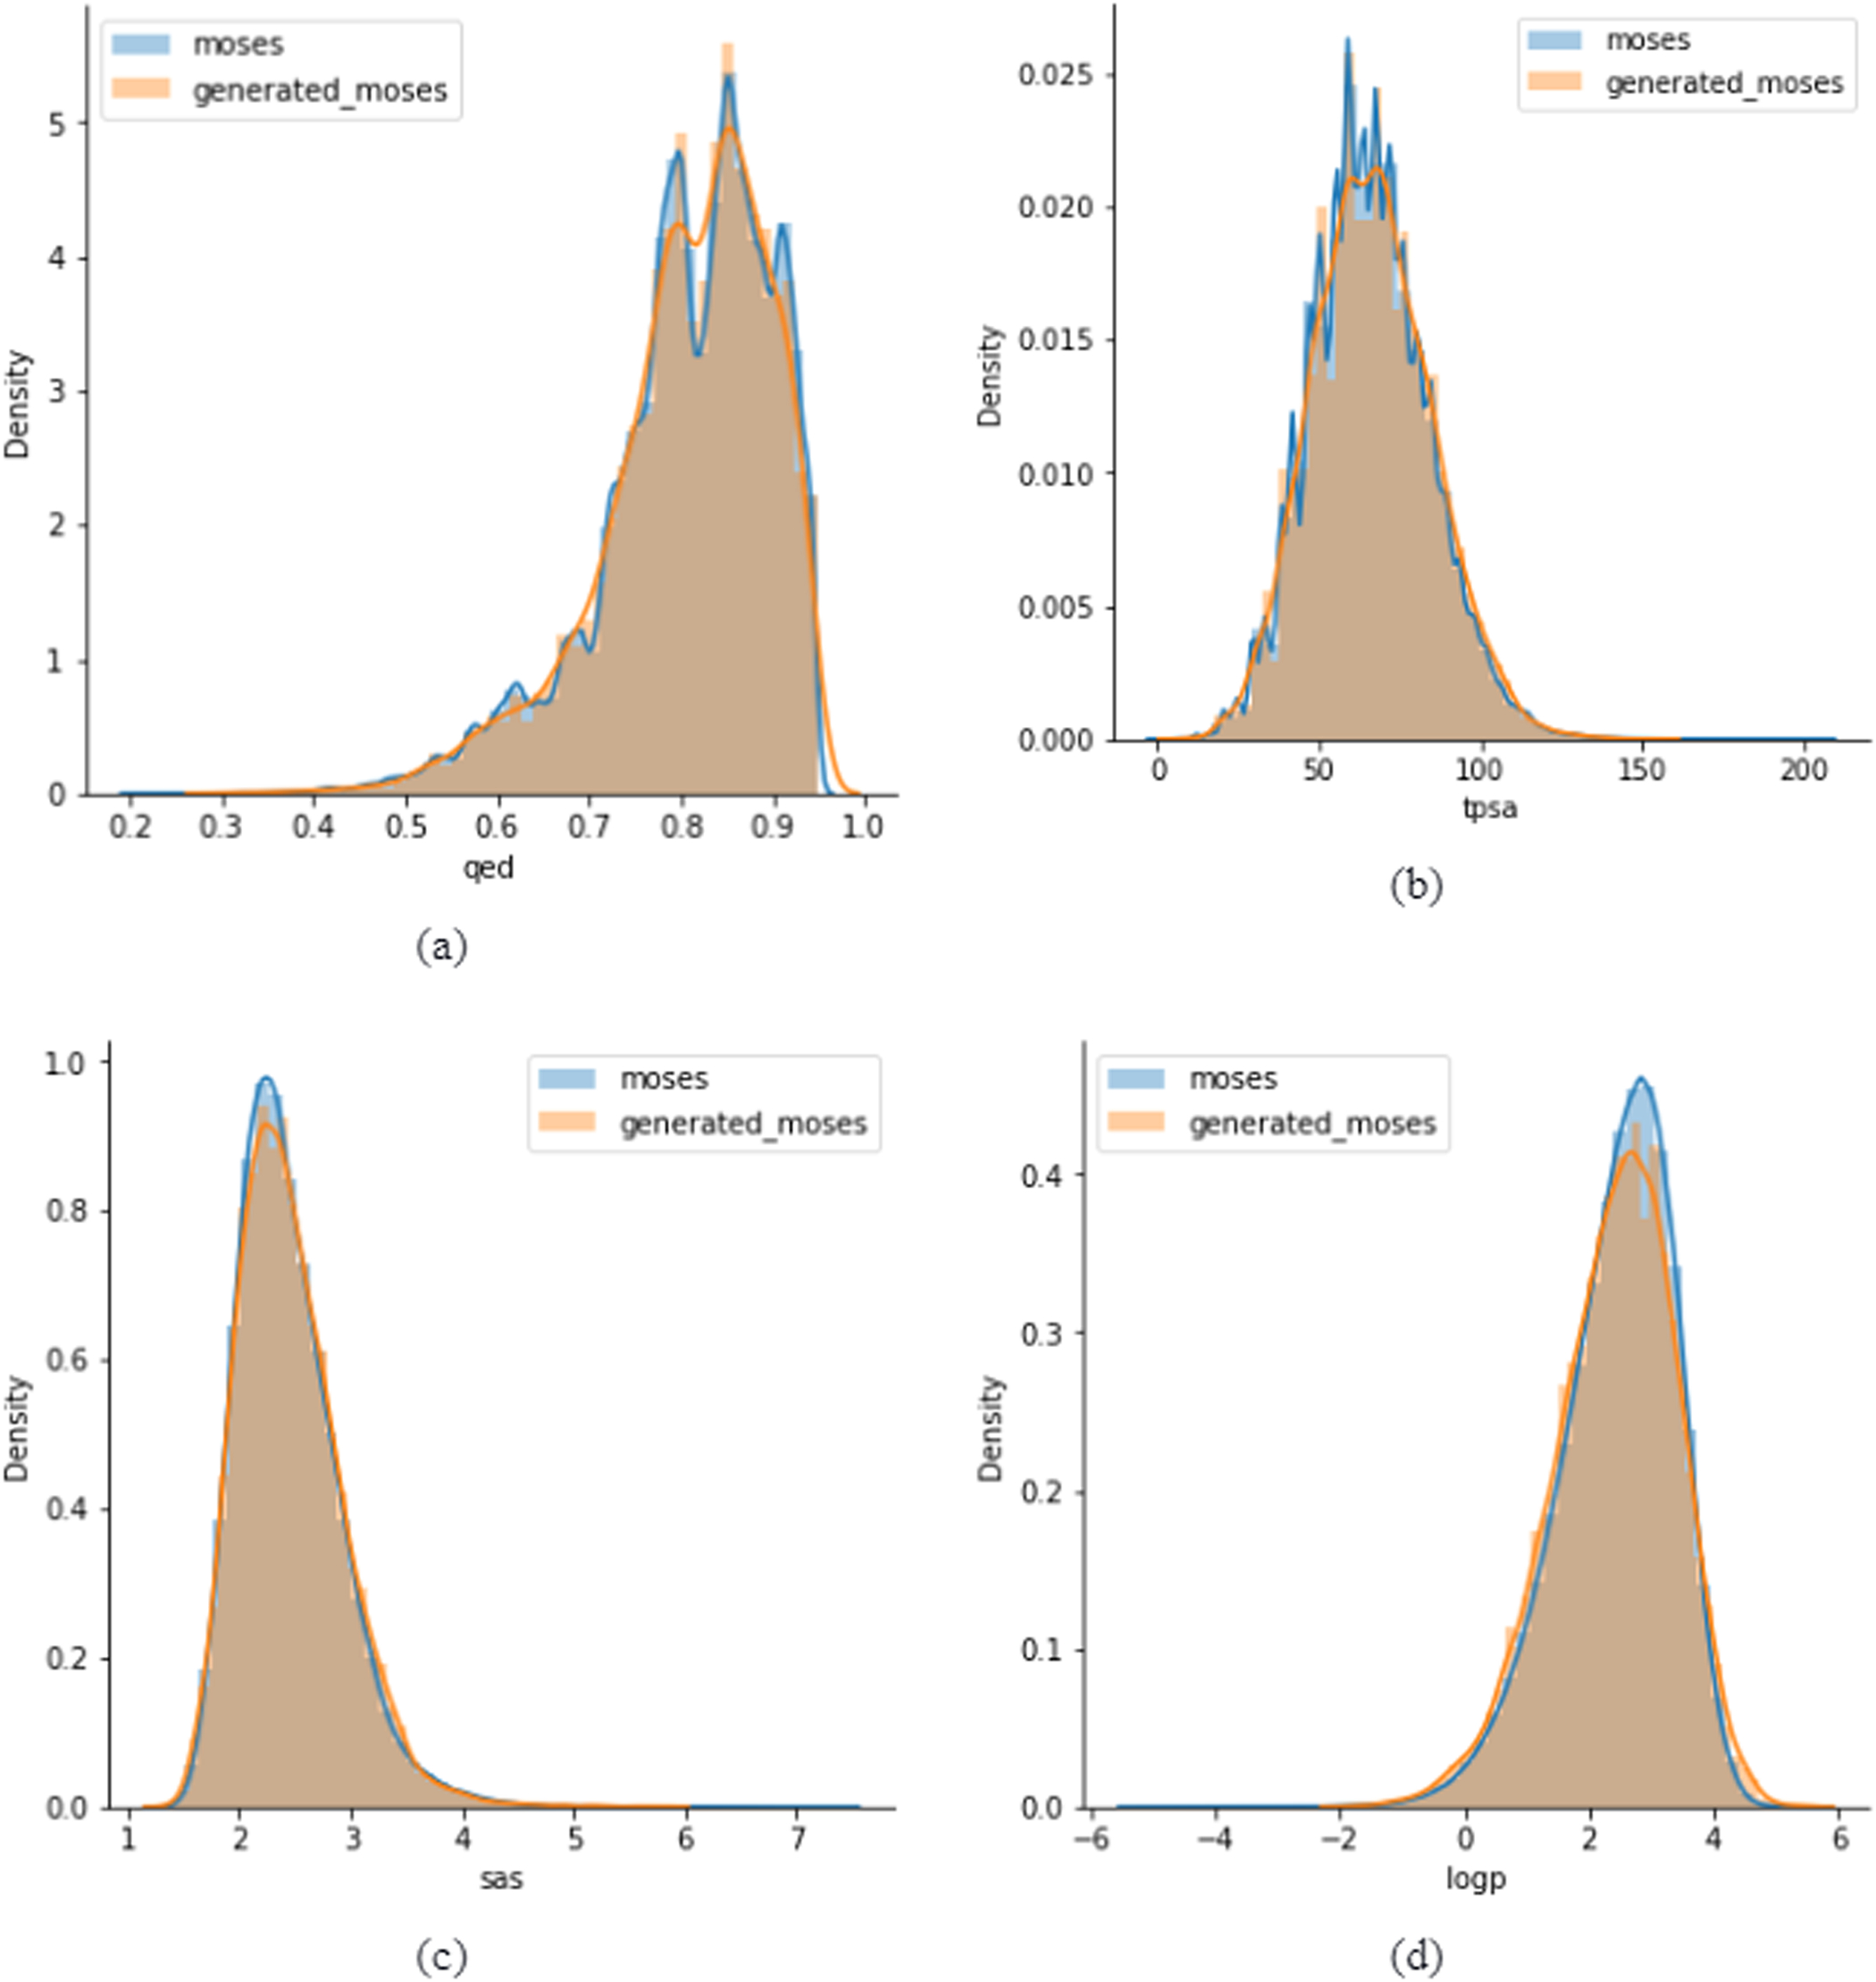
\includegraphics[width=\linewidth]{figures/3.png}
  \caption{MOSES 中分子的属性(QED、TPSA、SAS 和 logP)分布以及使用 MOSES 训练的具有相对注意力的模型生成的分子}
  \label{fig:3}
\end{figure}

图 \ref{fig:3} 说明了 MOSES 数据集与使用 MOSES 数据集训练所提出的模型后生成的药物之间的属性分布的比较。所提出的模型能够学习训练数据集的属性分布,从而生成在非条件生成期间表现出类似分布的分子。

\begin{table}[H]
  \centering
  \caption{使用 GuacaMol 进行非条件生成训练的生成模型之间的比较}
  \label{tab:2}
  \begin{tabular}{llll}
    \hline 模型       & 有效性   & 唯一性   & 新颖性   \\
    \hline VAE      & 0.870 & 0.999 & 0.974 \\
    AAE             & 0.822 & 1.0   & 0.998 \\
    ORGAN           & 0.379 & 0.841 & 0.687 \\
    SMILES LSTM     & 0.959 & 1.0   & 0.912 \\
    MolGPT          & 0.981 & 0.998 & 1.0   \\
    使用相对注意力的 MolGPT & 0.978 & 1.0   & 1.0   \\
    \hline
  \end{tabular}
\end{table}

表 \ref{tab:2} 提供了在 GuacaMol 数据集上训练的非条件生成的各种生成模型的全面比较。如表所示,具有标准注意力的 MolGPT 生成的药物的有效性达到 98.1\%,与训练集相比,所有药物都是新颖的。此外,当利用相对注意力时,该模型生成了 97.8\% 的有效药物,所有这些药物不仅新颖而且独特。

\begin{figure}[H]
  \centering
  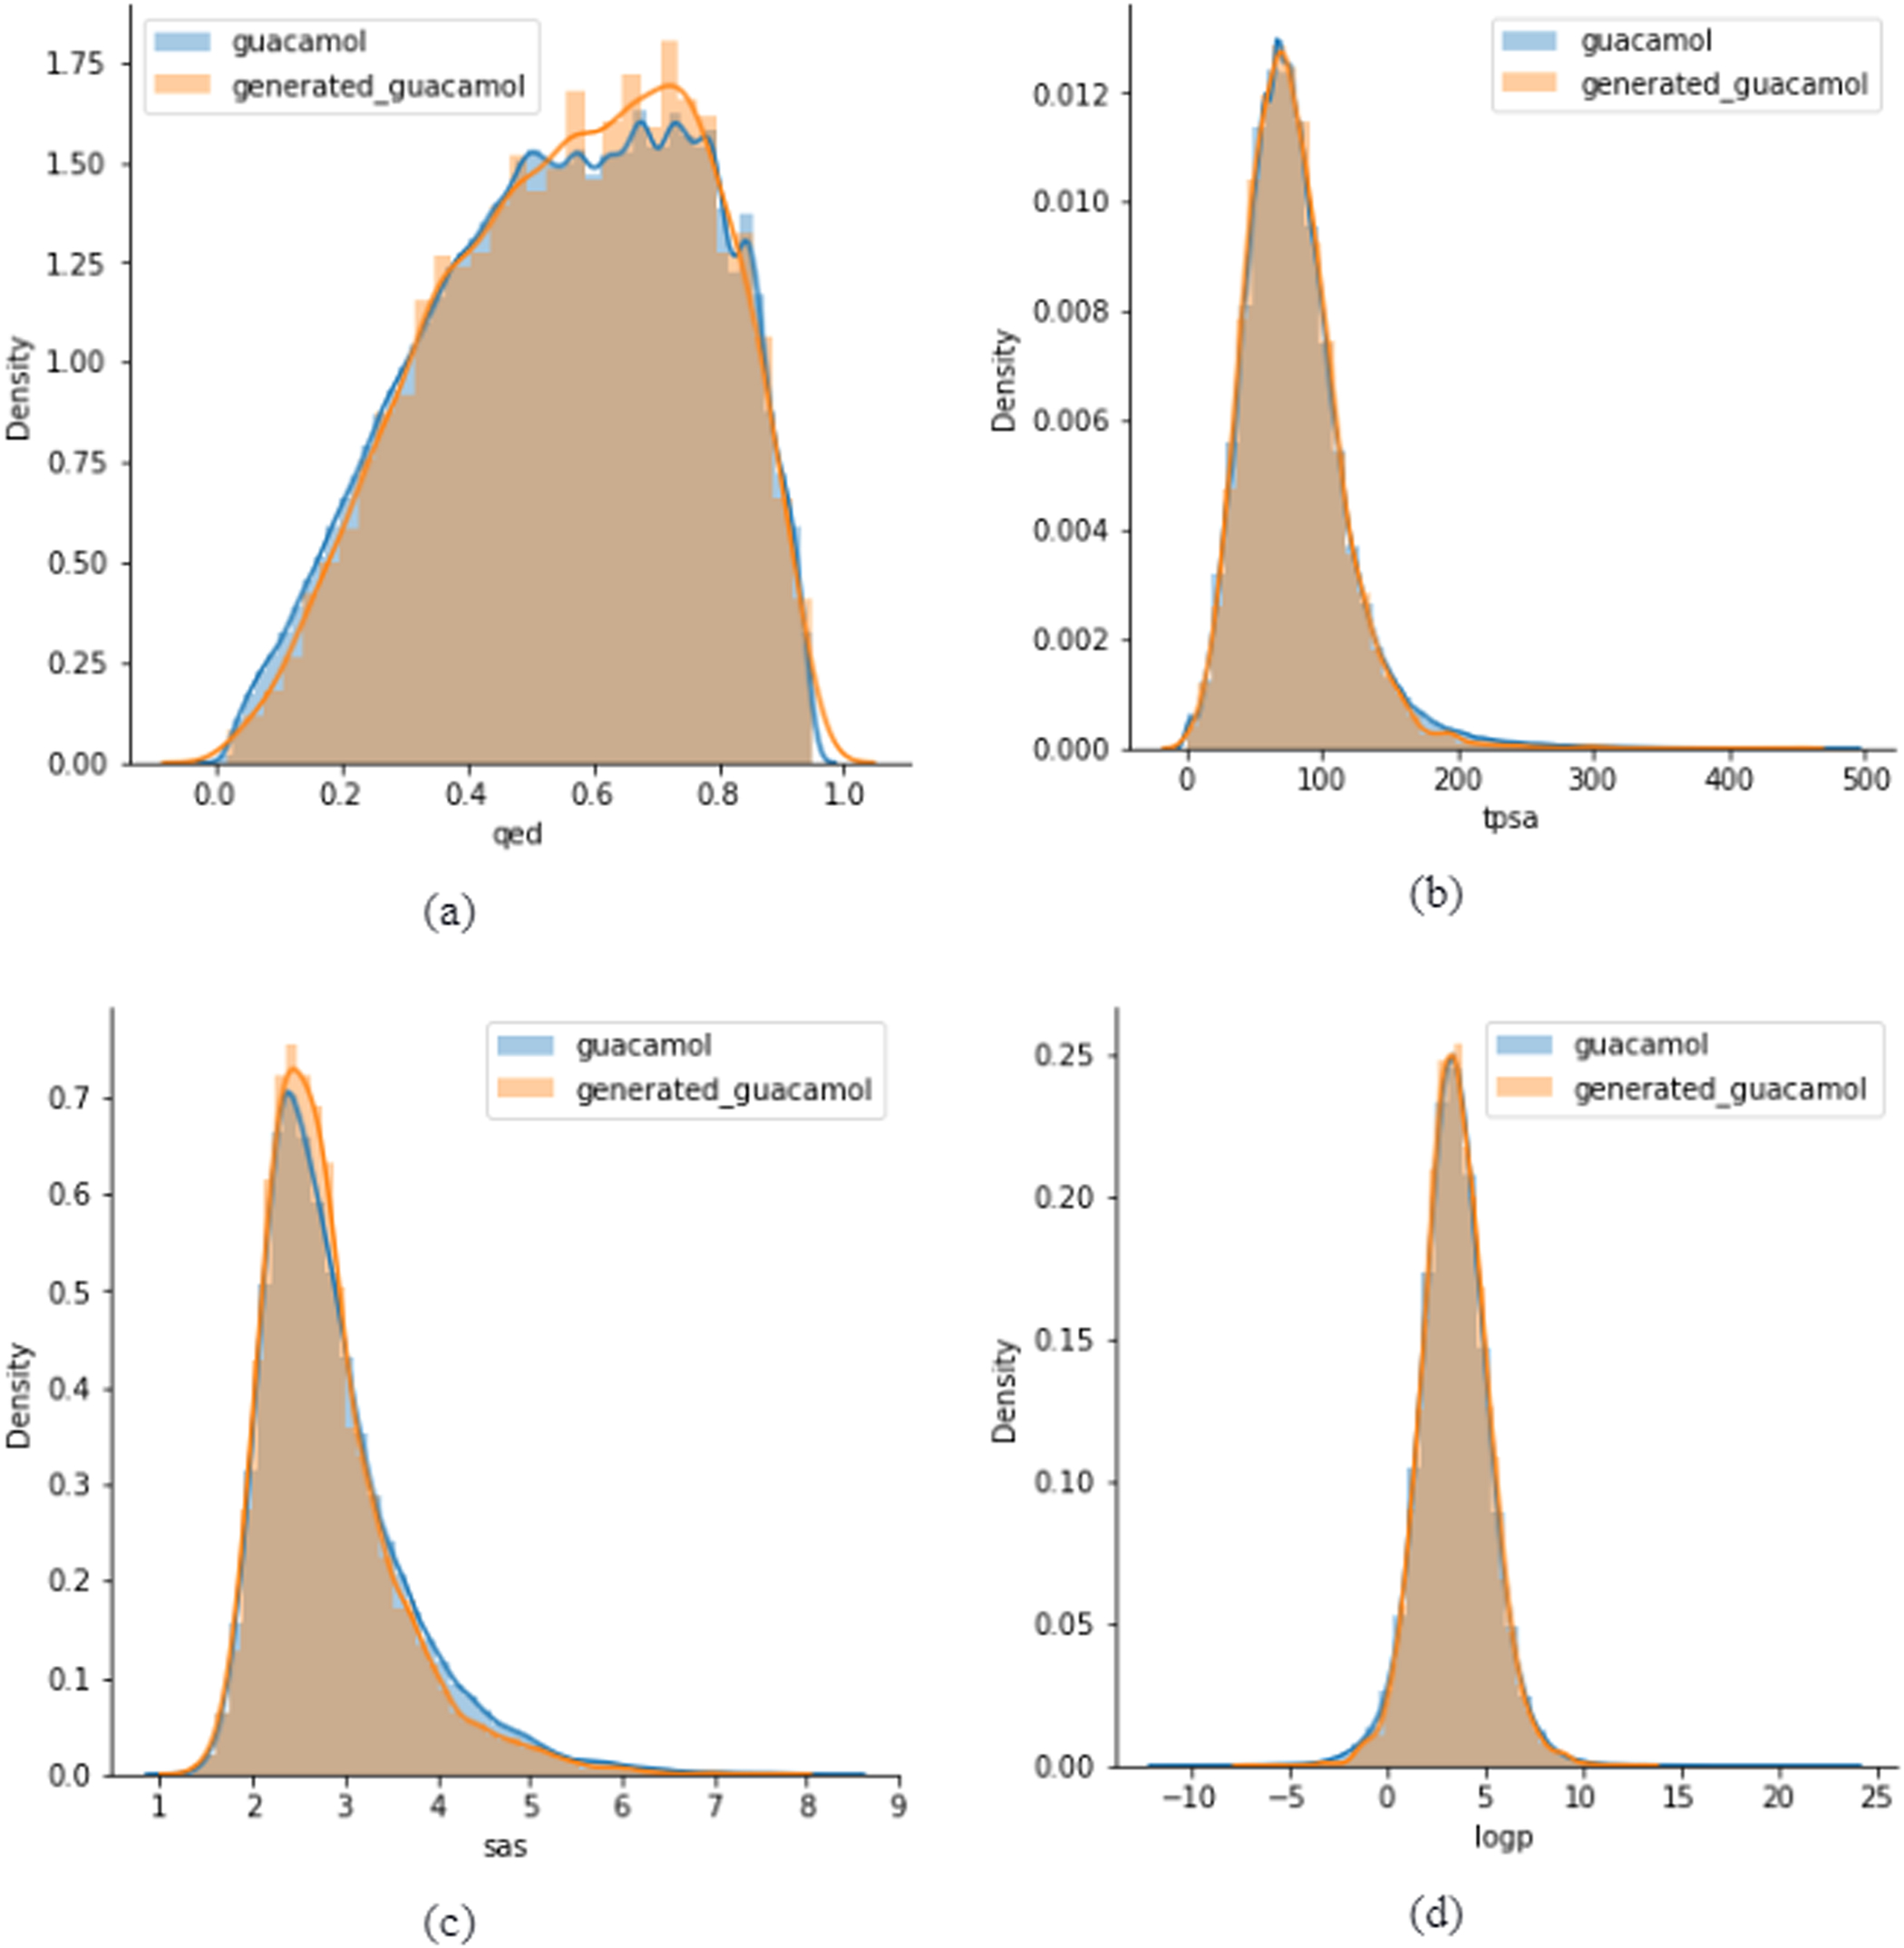
\includegraphics[width=\linewidth]{figures/4.png}
  \caption{GuacaMol 中分子的属性(QED、TPSA、SAS 和 logP)分布以及使用 GuacaMol 训练的具有相对注意力的模型生成的分子}
  \label{fig:4}
\end{figure}

图 \ref{fig:4} 比较了生成的药物和 GuacaMol 数据集的属性分布。模型预测的分子中 97.8\% 被识别为有效药物。所提出的模型证明了其从训练数据集中掌握和学习属性分布模式的能力。因此,在非条件生成过程中,模型生成的分子与训练数据集中观察到的分布非常相似。

\begin{table}[H]
  \centering
  \caption{GuacaMol 上训练标准注意力的分子条件生成的不同指标的比较}
  \label{tab:3}
  \begin{tabular}{llll}
    \hline 条件   & 有效性   & 唯一性   & 新颖性 \\
    \hline TPSA & 0.972 & 0.996 & 1.0 \\
    logP        & 0.971 & 0.998 & 1.0 \\
    SAS         & 0.977 & 0.995 & 1.0 \\
    QED         & 0.975 & 0.998 & 1.0 \\
    \hline
  \end{tabular}
\end{table}

\begin{table}[H]
  \centering
  \caption{GuacaMol 上训练的相对注意力的分子条件生成的不同指标的比较}
  \label{tab:4}
  \begin{tabular}{llll}
    \hline 条件   & 有效性   & 唯一性   & 新颖性 \\
    \hline TPSA & 0.982 & 0.999 & 1.0 \\
    log  P      & 0.969 & 1.0   & 1.0 \\
    SAS         & 0.986 & 0.997 & 1.0 \\
    QED         & 0.950 & 0.999 & 1.0 \\
    \hline
  \end{tabular}
\end{table}

当使用 GuacaMol 数据集评估具有标准注意力的 MolGPT(表 \ref{tab:3})和具有相对注意力的 MolGPT(表 \ref{tab:4})对于条件生成的性能时,在使用相对注意力的所有条件生成中观察到唯一性的适度增强。

为了评估模型在特定目标数据集上的性能,从 ExCAPEDB 中提取了两个数据集,即 HTR1A 和 S1PR1。这些数据集包含大约 72,000 个 SMILES 表达式。 MolGPT 在每个数据集上分别进行了 10 个时期的训练,同时采用了标准和相对注意机制。

\begin{table}[H]
  \centering
  \caption{S1PR1 上训练的标准注意力模型的不同指标的比较}
  \label{tab:5}
  \begin{tabular}{llll}
    \hline 条件  & 有效性   & 唯一性   & 新颖性 \\
    \hline 无条件 & 0.879 & 0.996 & 1   \\
    logP       & 0.868 & 0.994 & 1   \\
    SAS        & 0.852 & 0.997 & 1   \\
    TPSA       & 0.862 & 0.996 & 1   \\
    QED        & 0.906 & 0.976 & 1   \\
    \hline
  \end{tabular}
\end{table}


\begin{table}[H]
  \centering
  \caption{S1PR1 上训练的相对注意力模型的不同指标的比较}
  \label{tab:6}
  \begin{tabular}{llll}
    \hline 条件  & 有效性   & 唯一性   & 新颖性 \\
    \hline 无条件 & 0.87  & 0.99  & 1   \\
    logP       & 0.844 & 0.983 & 1   \\
    SAS        & 0.85  & 0.992 & 1   \\
    TPSA       & 0.855 & 0.989 & 1   \\
    QED        & 0.89  & 0.989 & 1   \\
    \hline
  \end{tabular}
\end{table}

\begin{table}[H]
  \centering
  \caption{HTR1A 上训练的标准注意力模型的不同指标的比较}
  \label{tab:7}
  \begin{tabular}{llll}
    \hline 条件  & 有效性   & 唯一性   & 新颖性 \\
    \hline 无条件 & 0.876 & 0.997 & 1   \\
    logP       & 0.801 & 0.999 & 1   \\
    SAS        & 0.849 & 0.999 & 1   \\
    TPSA       & 0.835 & 0.996 & 1   \\
    QED        & 0.878 & 0.998 & 1   \\
    \hline
  \end{tabular}
\end{table}

\begin{table}[H]
  \centering
  \caption{HTR1A 上训练的相对注意力模型的不同指标的比较}
  \label{tab:8}
  \begin{tabular}{llll}
    \hline 条件  & 有效性   & 唯一性   & 新颖性 \\
    \hline 无条件 & 0.81  & 0.991 & 1   \\
    logP       & 0.757 & 0.996 & 1   \\
    SAS        & 0.817 & 0.994 & 1   \\
    TPSA       & 0.836 & 0.99  & 1   \\
    QED        & 0.855 & 0.991 & 1   \\
    \hline
  \end{tabular}
\end{table}

\begin{figure}[H]
  \centering
  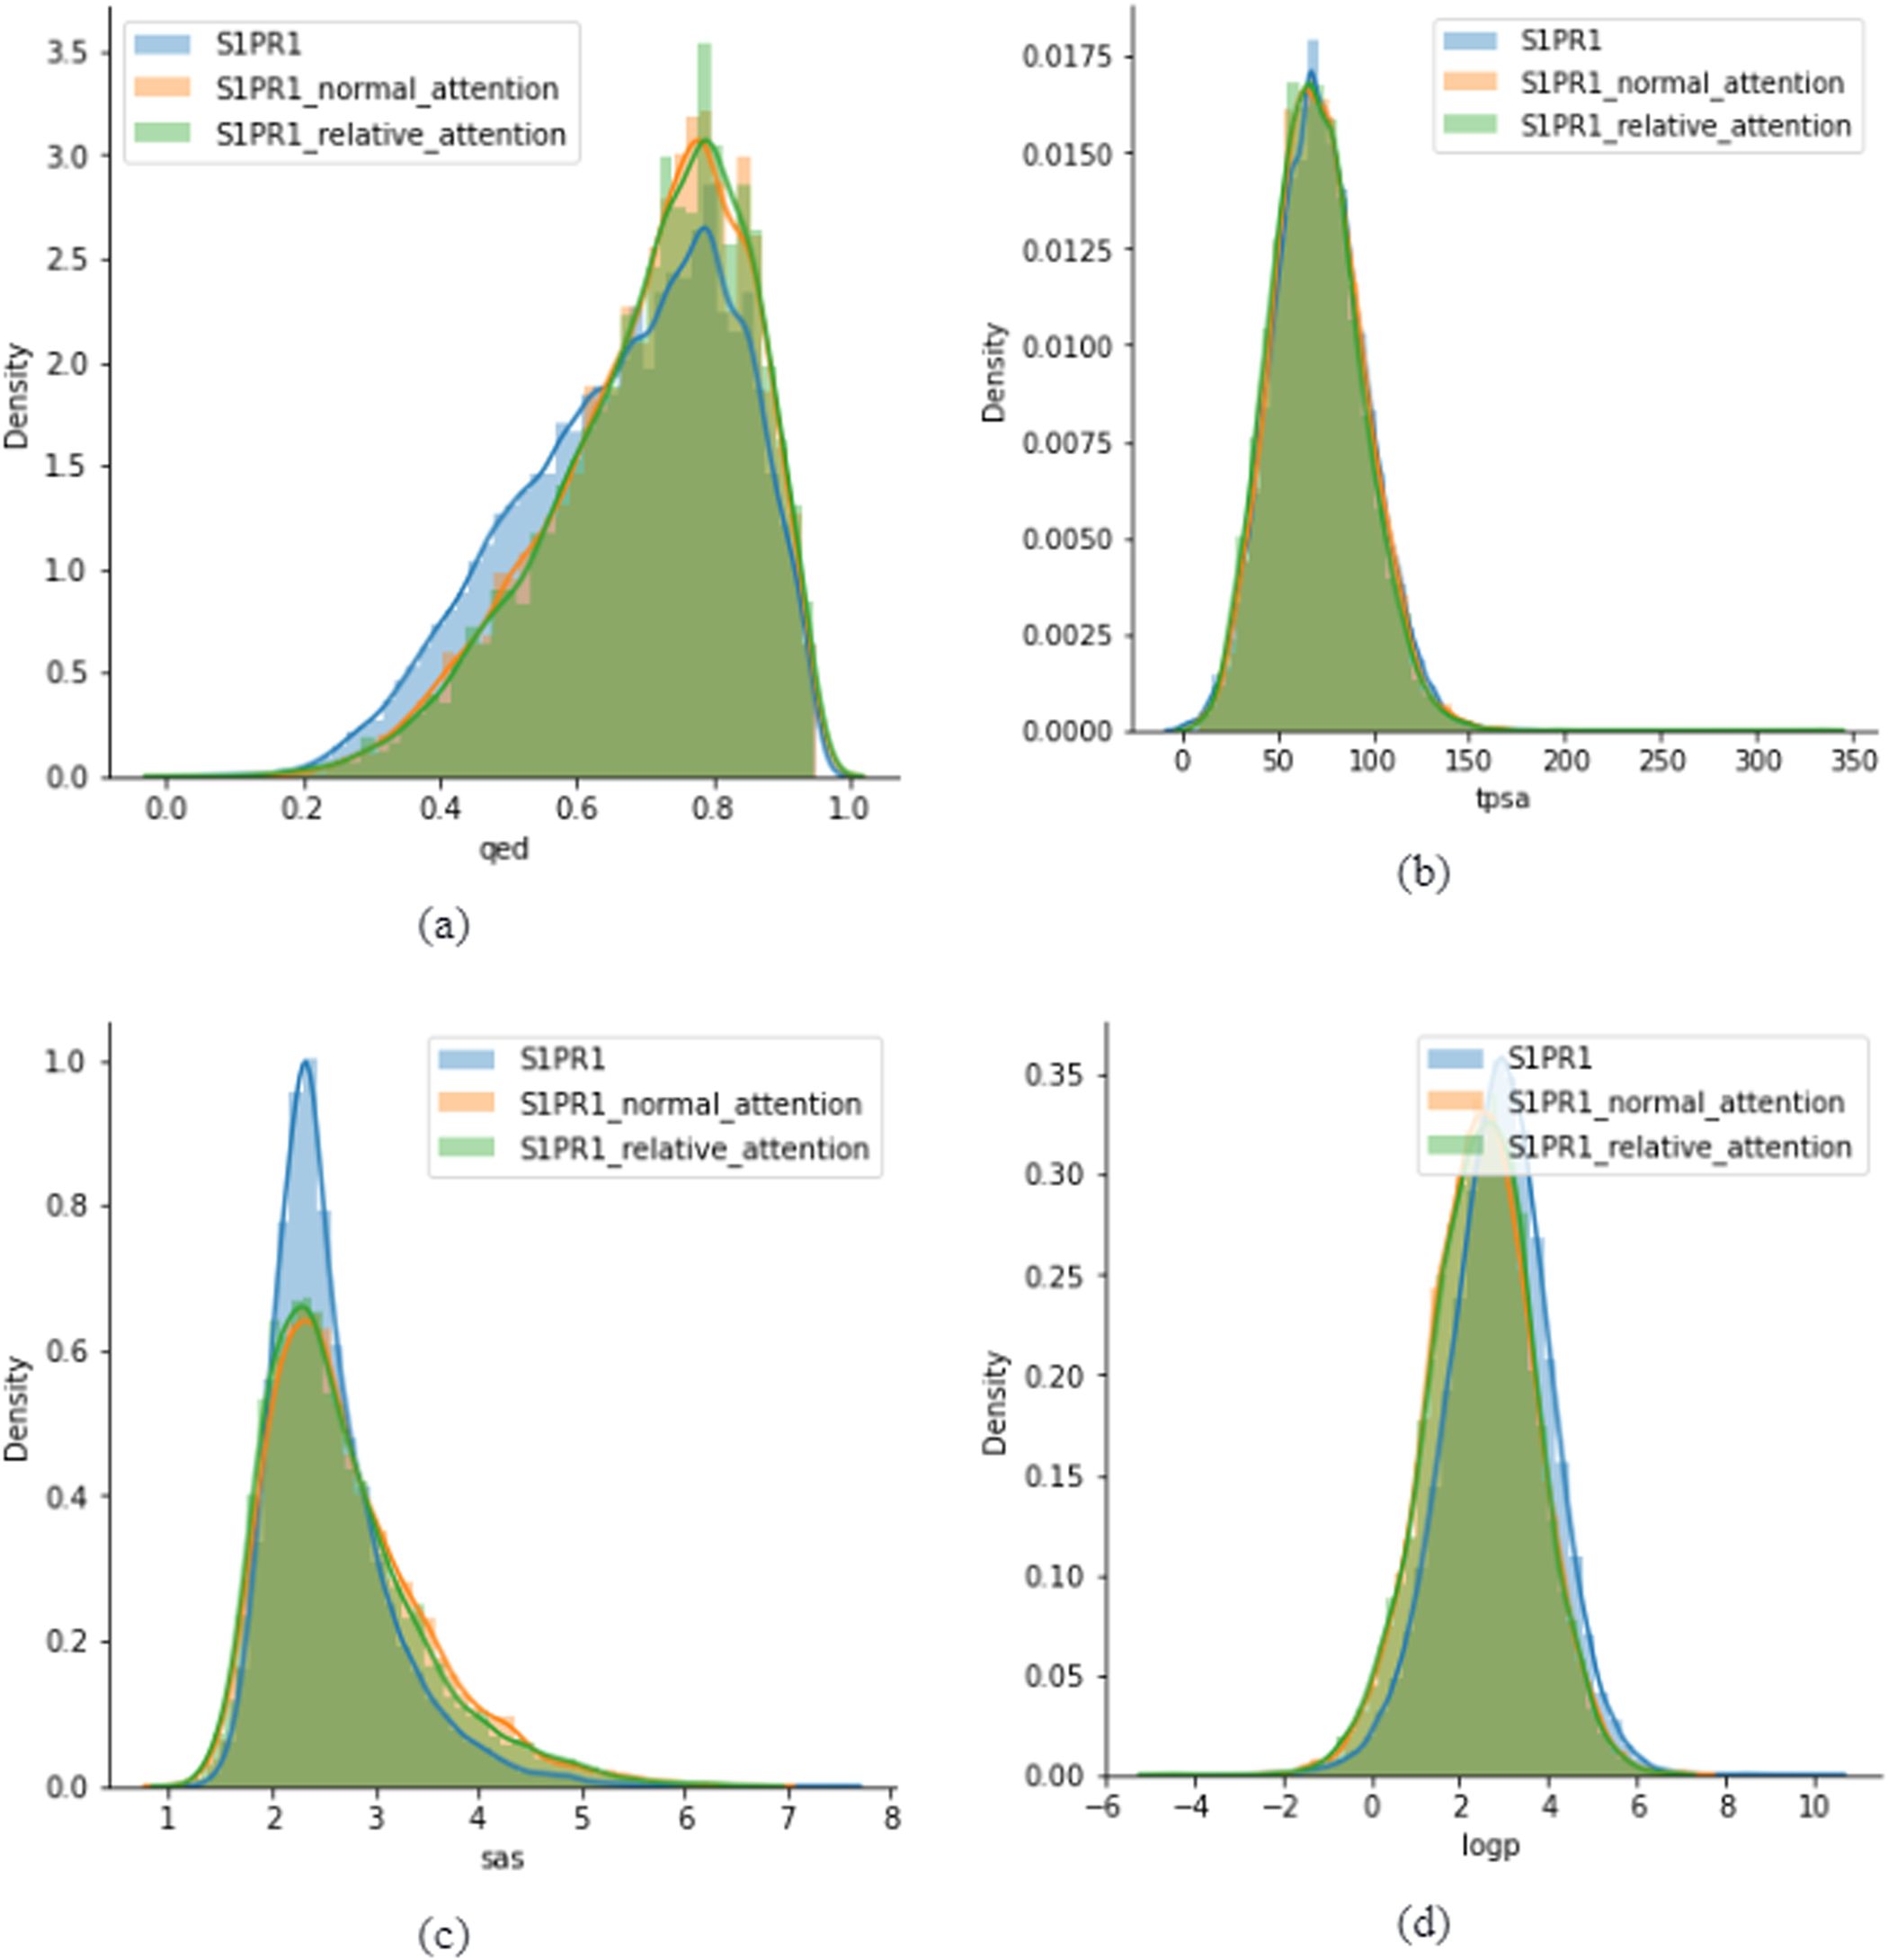
\includegraphics[width=\linewidth]{figures/5.png}
  \caption{S1PR1 中的分子以及具有标准注意力和相对注意力的模型生成的分子的属性(QED、TPSA、SAS 和 logP)分布}
  \label{fig:5}
\end{figure}

\begin{figure}[H]
  \centering
  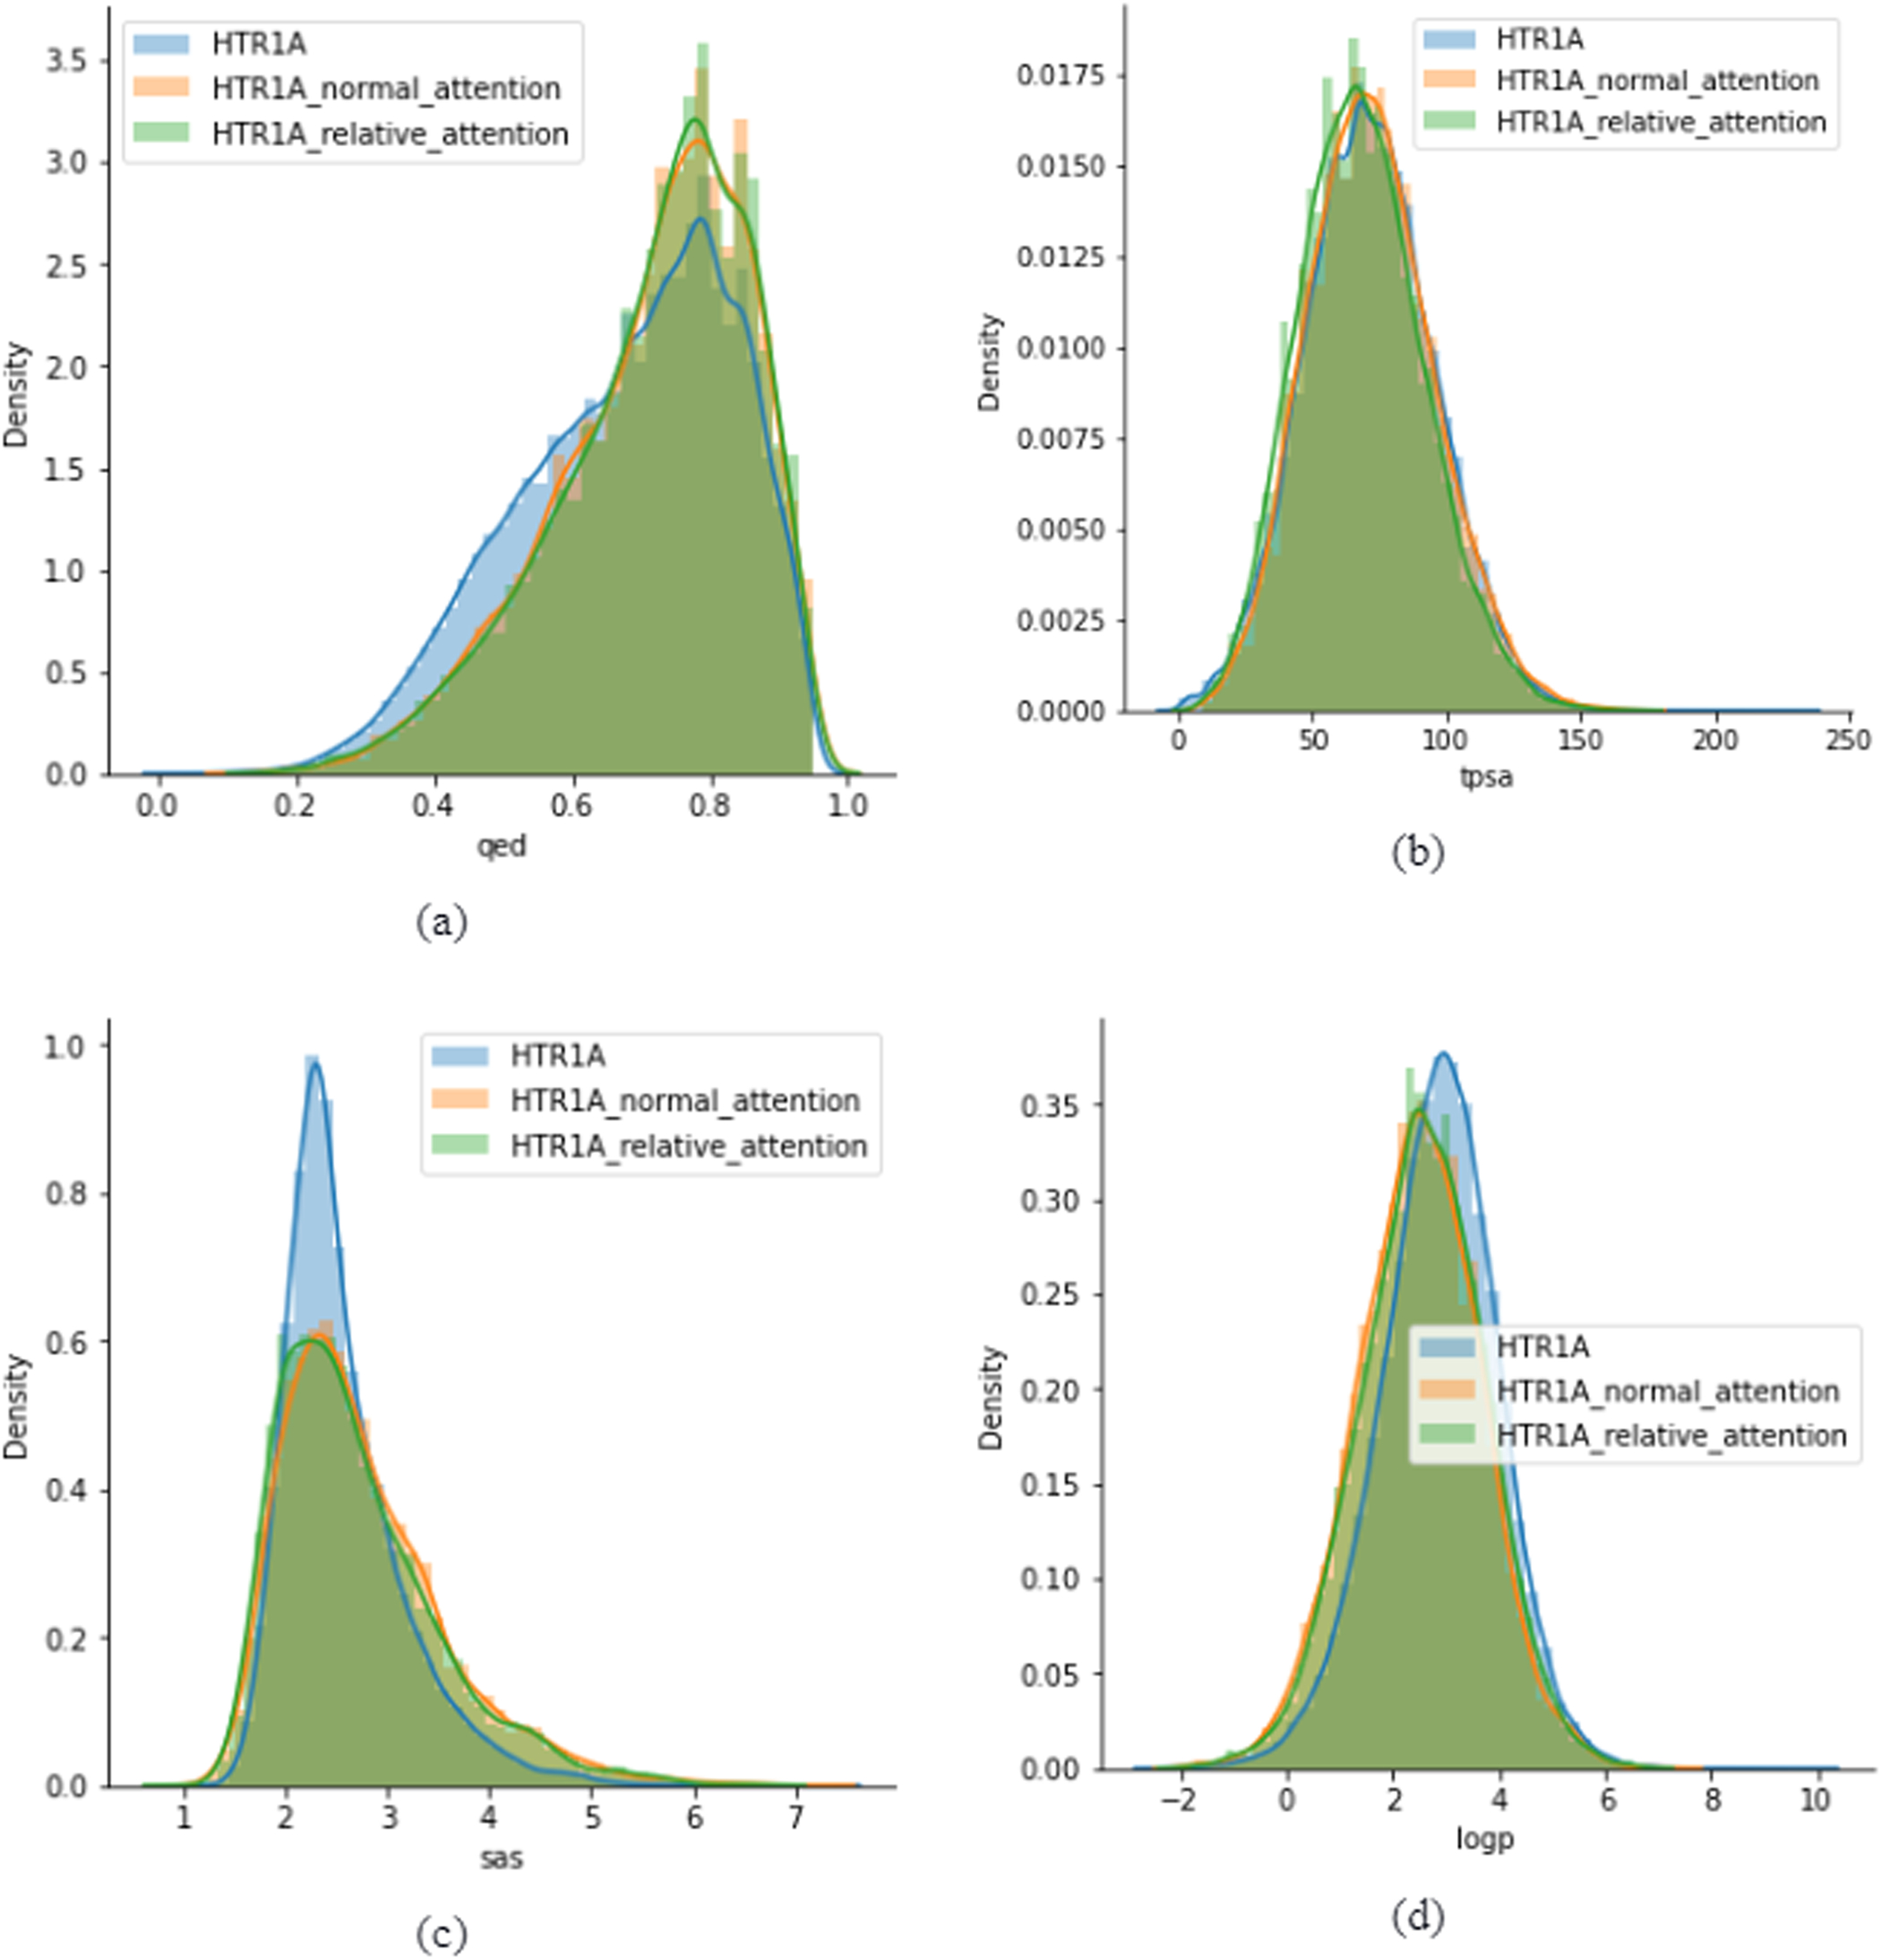
\includegraphics[width=\linewidth]{figures/6.png}
  \caption{HTR1A 数据集中分子的属性(QED、TPSA、SAS 和 logP)分布以及使用标准注意力和相对注意力训练的模型生成的分子}
  \label{fig:6}
\end{figure}

表 \ref{tab:5} 和表 \ref{tab:6} 比较了 S1PR1 数据集中标准注意力和相对注意力的表现,而表 \ref{tab:7} 和表 \ref{tab:8} 提供了 HTR1A 数据集的类似比较。图 \ref{fig:5} 和图 \ref{fig:6} 展示了S1PR1和HTR1A数据集中分子的属性分布,以及使用标准和相对注意力的模型生成的分子的属性分布。这两个模型在标准和相对关注的情况下,成功生成了具有与训练集非常相似的属性分布的分子。然而,与具有相对注意力的模型相比,具有标准注意力的 MolGPT 预测的有效分子数量略多。

HTR1A 和 S1PR1 数据集分别采样了 3400 和 800 个 SMILES,以证明相对注意力在较小数据集上的性能。后来它们被分成训练集和测试集。由于数据集大小有限,模型无法学习 SMILES 的语法。为了克服这个问题,使用了迁移学习技术。当使用迁移学习将模型的性能与较小的数据集进行比较时,通过调整相对注意力(与标准注意力相比)可以观察到显着的改进。使用 MOSES 数据集分别训练具有相对注意力的模型和具有标准注意力的模型。权重用于训练特定于目标的较小数据集。由于训练数据集较小,该模型配置为仅预测 1000 个分子。

\begin{table}[H]
  \centering
  \caption{使用迁移学习对采样 S1PR1 非条件生成训练的标准注意力模型和相对注意力模型的比较}
  \label{tab:9}
  \begin{tabular}{llll}
    \hline 模型       & 有效性   & 唯一性   & 新颖性   \\
    \hline ModelGPT & 0.47  & 0.94  & 0.996 \\
    使用相对注意力的 MolGPT & 0.588 & 0.958 & 0.979 \\
    \hline
  \end{tabular}
\end{table}

表 \ref{tab:9} 提供了使用标准注意力和使用采样的 S1PR1 数据集和迁移学习进行非条件生成的相对注意力进行训练的性能比较。当进行标准注意力训练时,只有 47\% 的预测分子被识别为有效药物。然而,当进行相对关注的训练时,该有效性百分比增加到 58.8\%,从而显着提高 11.8\%。

\begin{table}[H]
  \centering
  \caption{使用迁移学习在采样 S1PR1 上训练条件生成的相对注意力模型的不同指标的比较}
  \label{tab:10}
  \begin{tabular}{llll}
    \hline 条件 & 有效性   & 唯一性   & 新颖性   \\
    logP      & 0.724 & 0.86  & 0.984 \\
    TPSA      & 0.739 & 0.794 & 0.988 \\
    SAS       & 0.708 & 0.99  & 0.99  \\
    QED       & 0.685 & 0.991 & 0.99  \\
    \hline
  \end{tabular}
\end{table}


\begin{figure}[H]
  \centering
  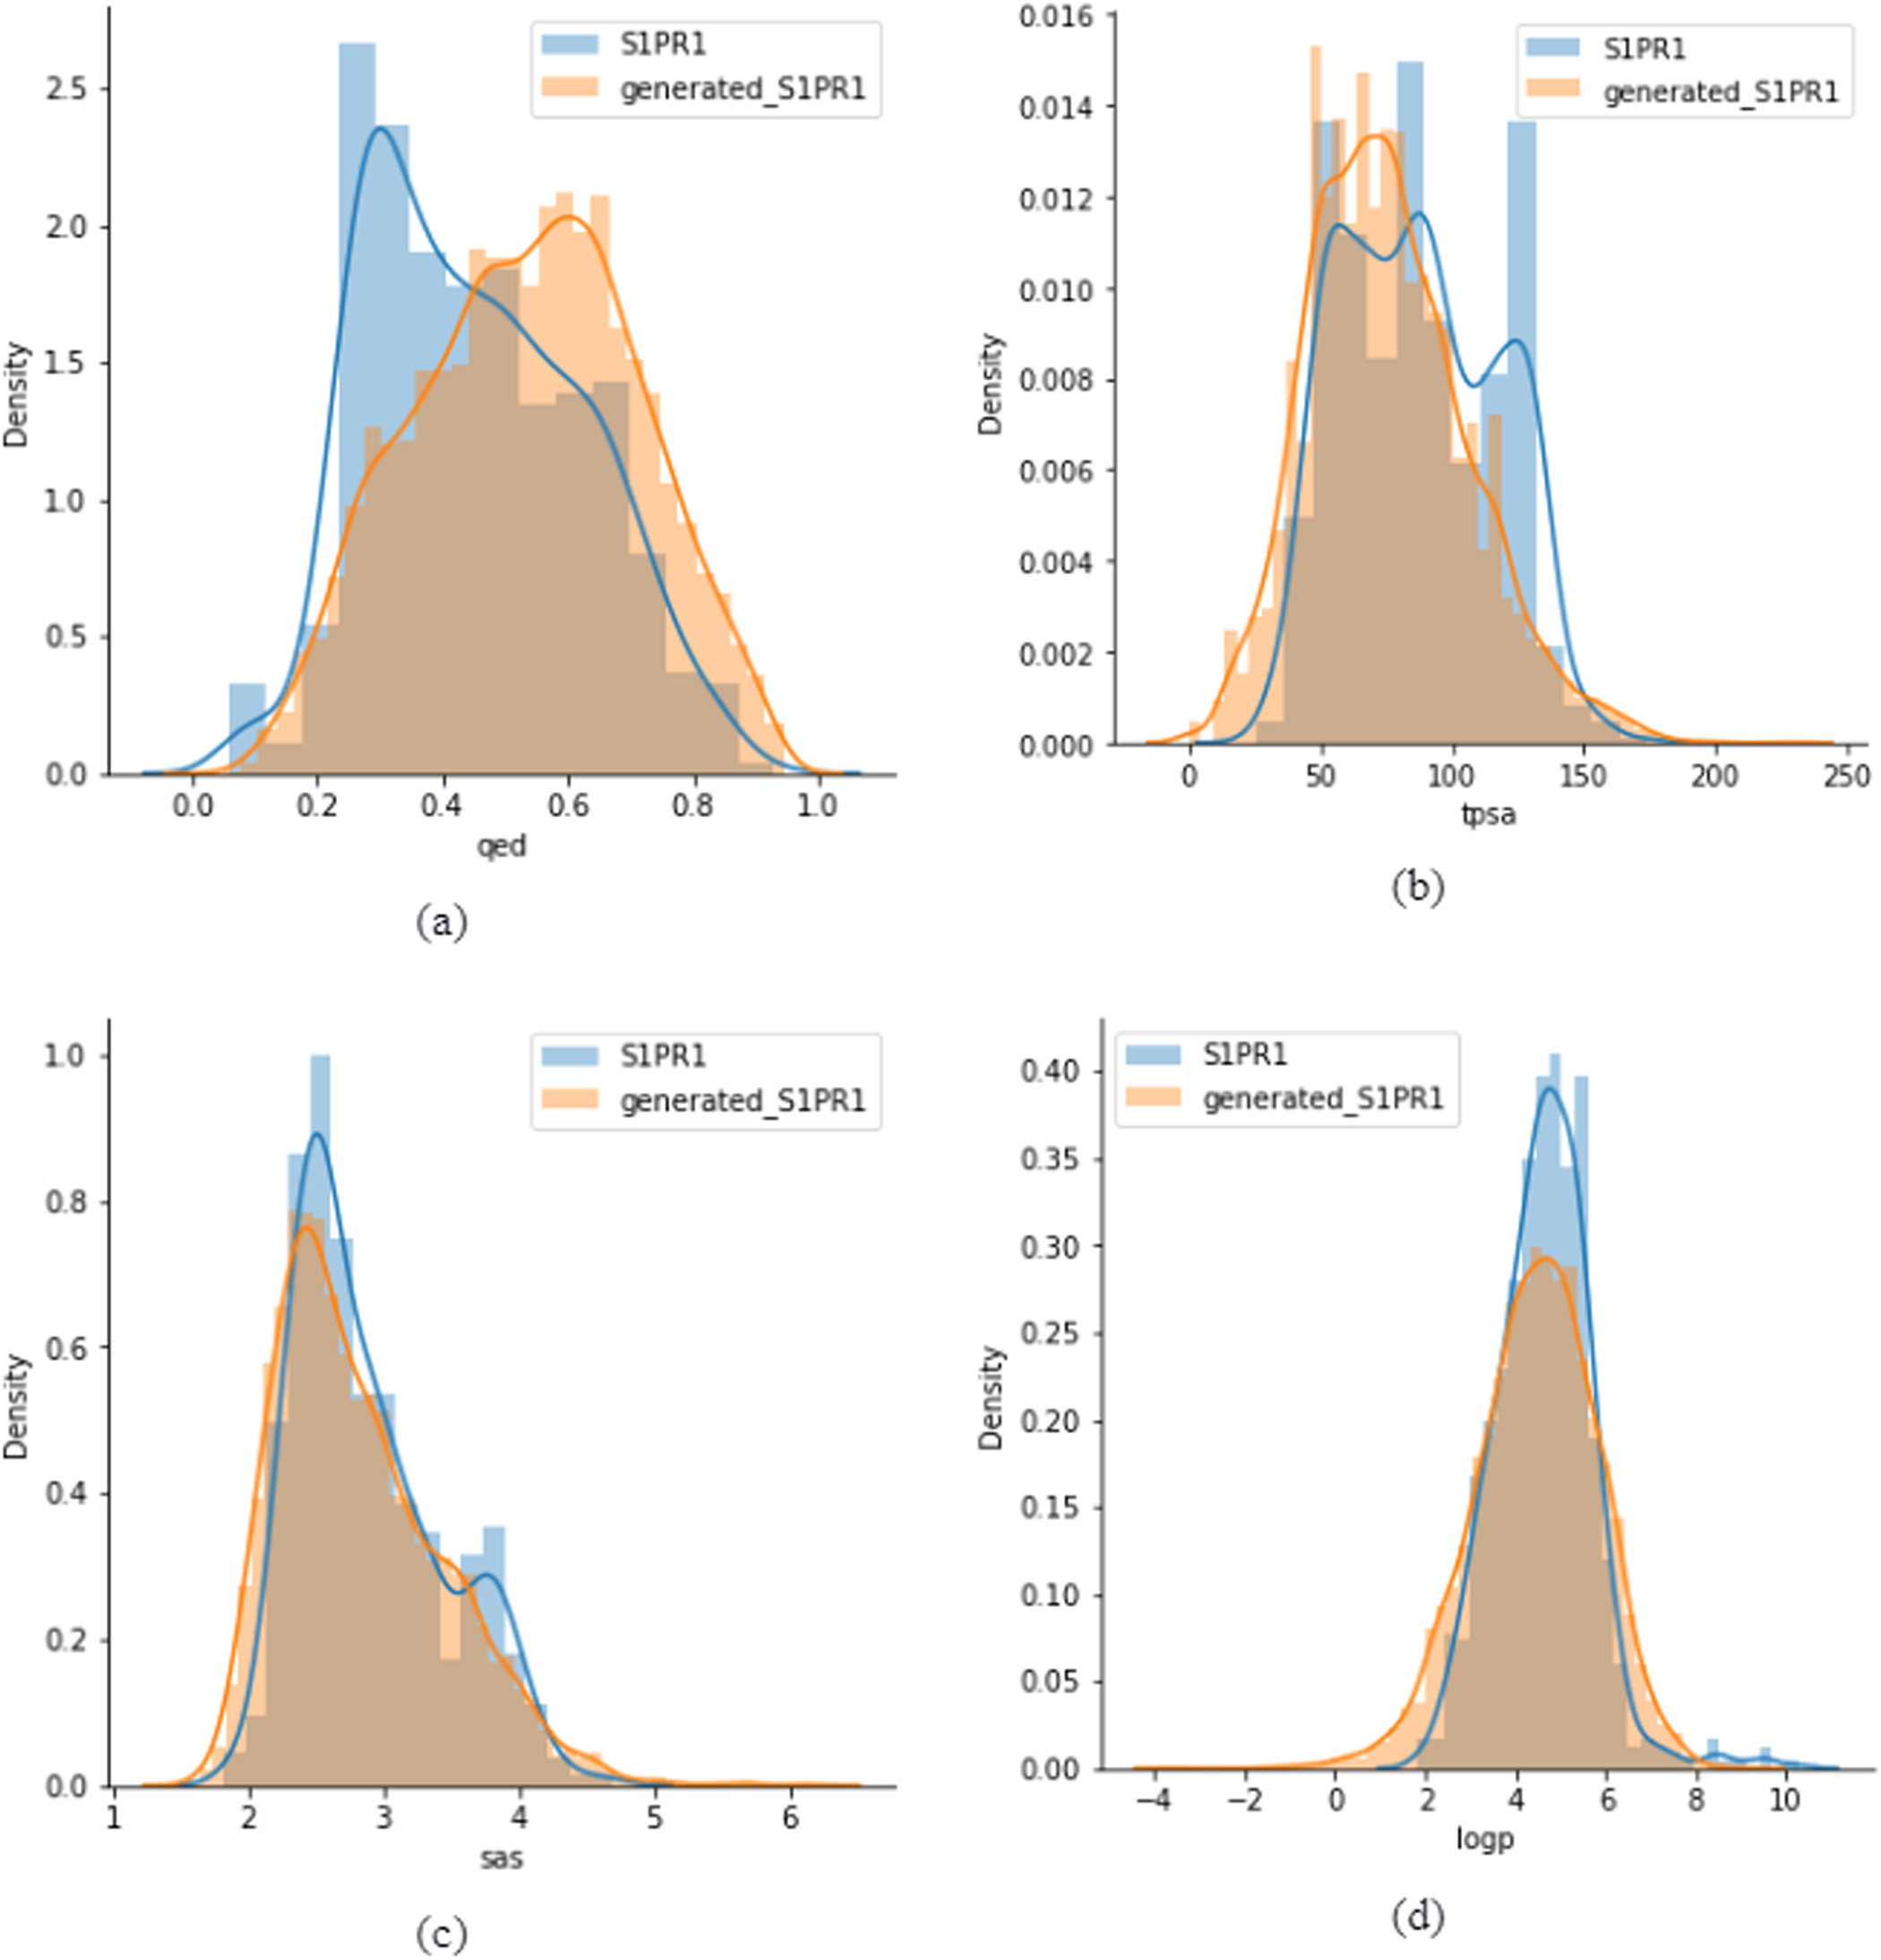
\includegraphics[width=\linewidth]{figures/7.png}
  \caption{采样的 S1PR1 中的分子和相对关注生成的分子的属性(QED、TPSA、SAS 和 logP)分布}
  \label{fig:7}
\end{figure}

在表 \ref{tab:10} 中,报告了使用采样的 S1PR1 数据集进行条件生成的具有相对关注的模型的性能。此外,图 \ref{fig:7} 直观地展示了采样的 S1PR1 数据集中分子的属性分布以及使用相对注意力生成的分子。

\begin{table}[H]
  \centering
  \caption{使用迁移学习使用采样 HTR1A 非条件生成训练的标准和相对注意力模型之间的比较}
  \label{tab:11}
  \begin{tabular}{llll}
    \hline 模型       & 有效性   & 唯一性   & 新颖性   \\
    \hline ModelGPT & 0.852 & 0.928 & 0.859 \\
    使用相对注意力的 MolGPT & 0.863 & 0.945 & 0.877 \\
    \hline
  \end{tabular}
\end{table}

表 \ref{tab:11} 展示了使用采样的 HTR1A 数据集和迁移学习进行非条件生成的标准注意力和相对注意力训练的模型之间的性能比较。采样数据集包含 3400 个 SMILES。具有标准注意力的 MolGPT 预测了 85.2\% 的有效药物。然而,当采用相对关注时,有效性增加到 86.3\%。

\begin{table}[H]
  \centering
  \caption{使用迁移学习使用采样 HTR1A 非条件生成训练的标准和相对注意力模型之间的比较}
  \label{tab:12}
  \begin{tabular}{llll}
    \hline 条件 & 有效性   & 唯一性   & 新颖性   \\
    logP      & 0.804 & 0.824 & 0.947 \\
    TPSA      & 0.878 & 0.706 & 0.946 \\
    SAS       & 0.861 & 0.684 & 0.934 \\
    QED       & 0.893 & 0.793 & 0.946 \\
    \hline
  \end{tabular}
\end{table}

\begin{figure}[H]
  \centering
  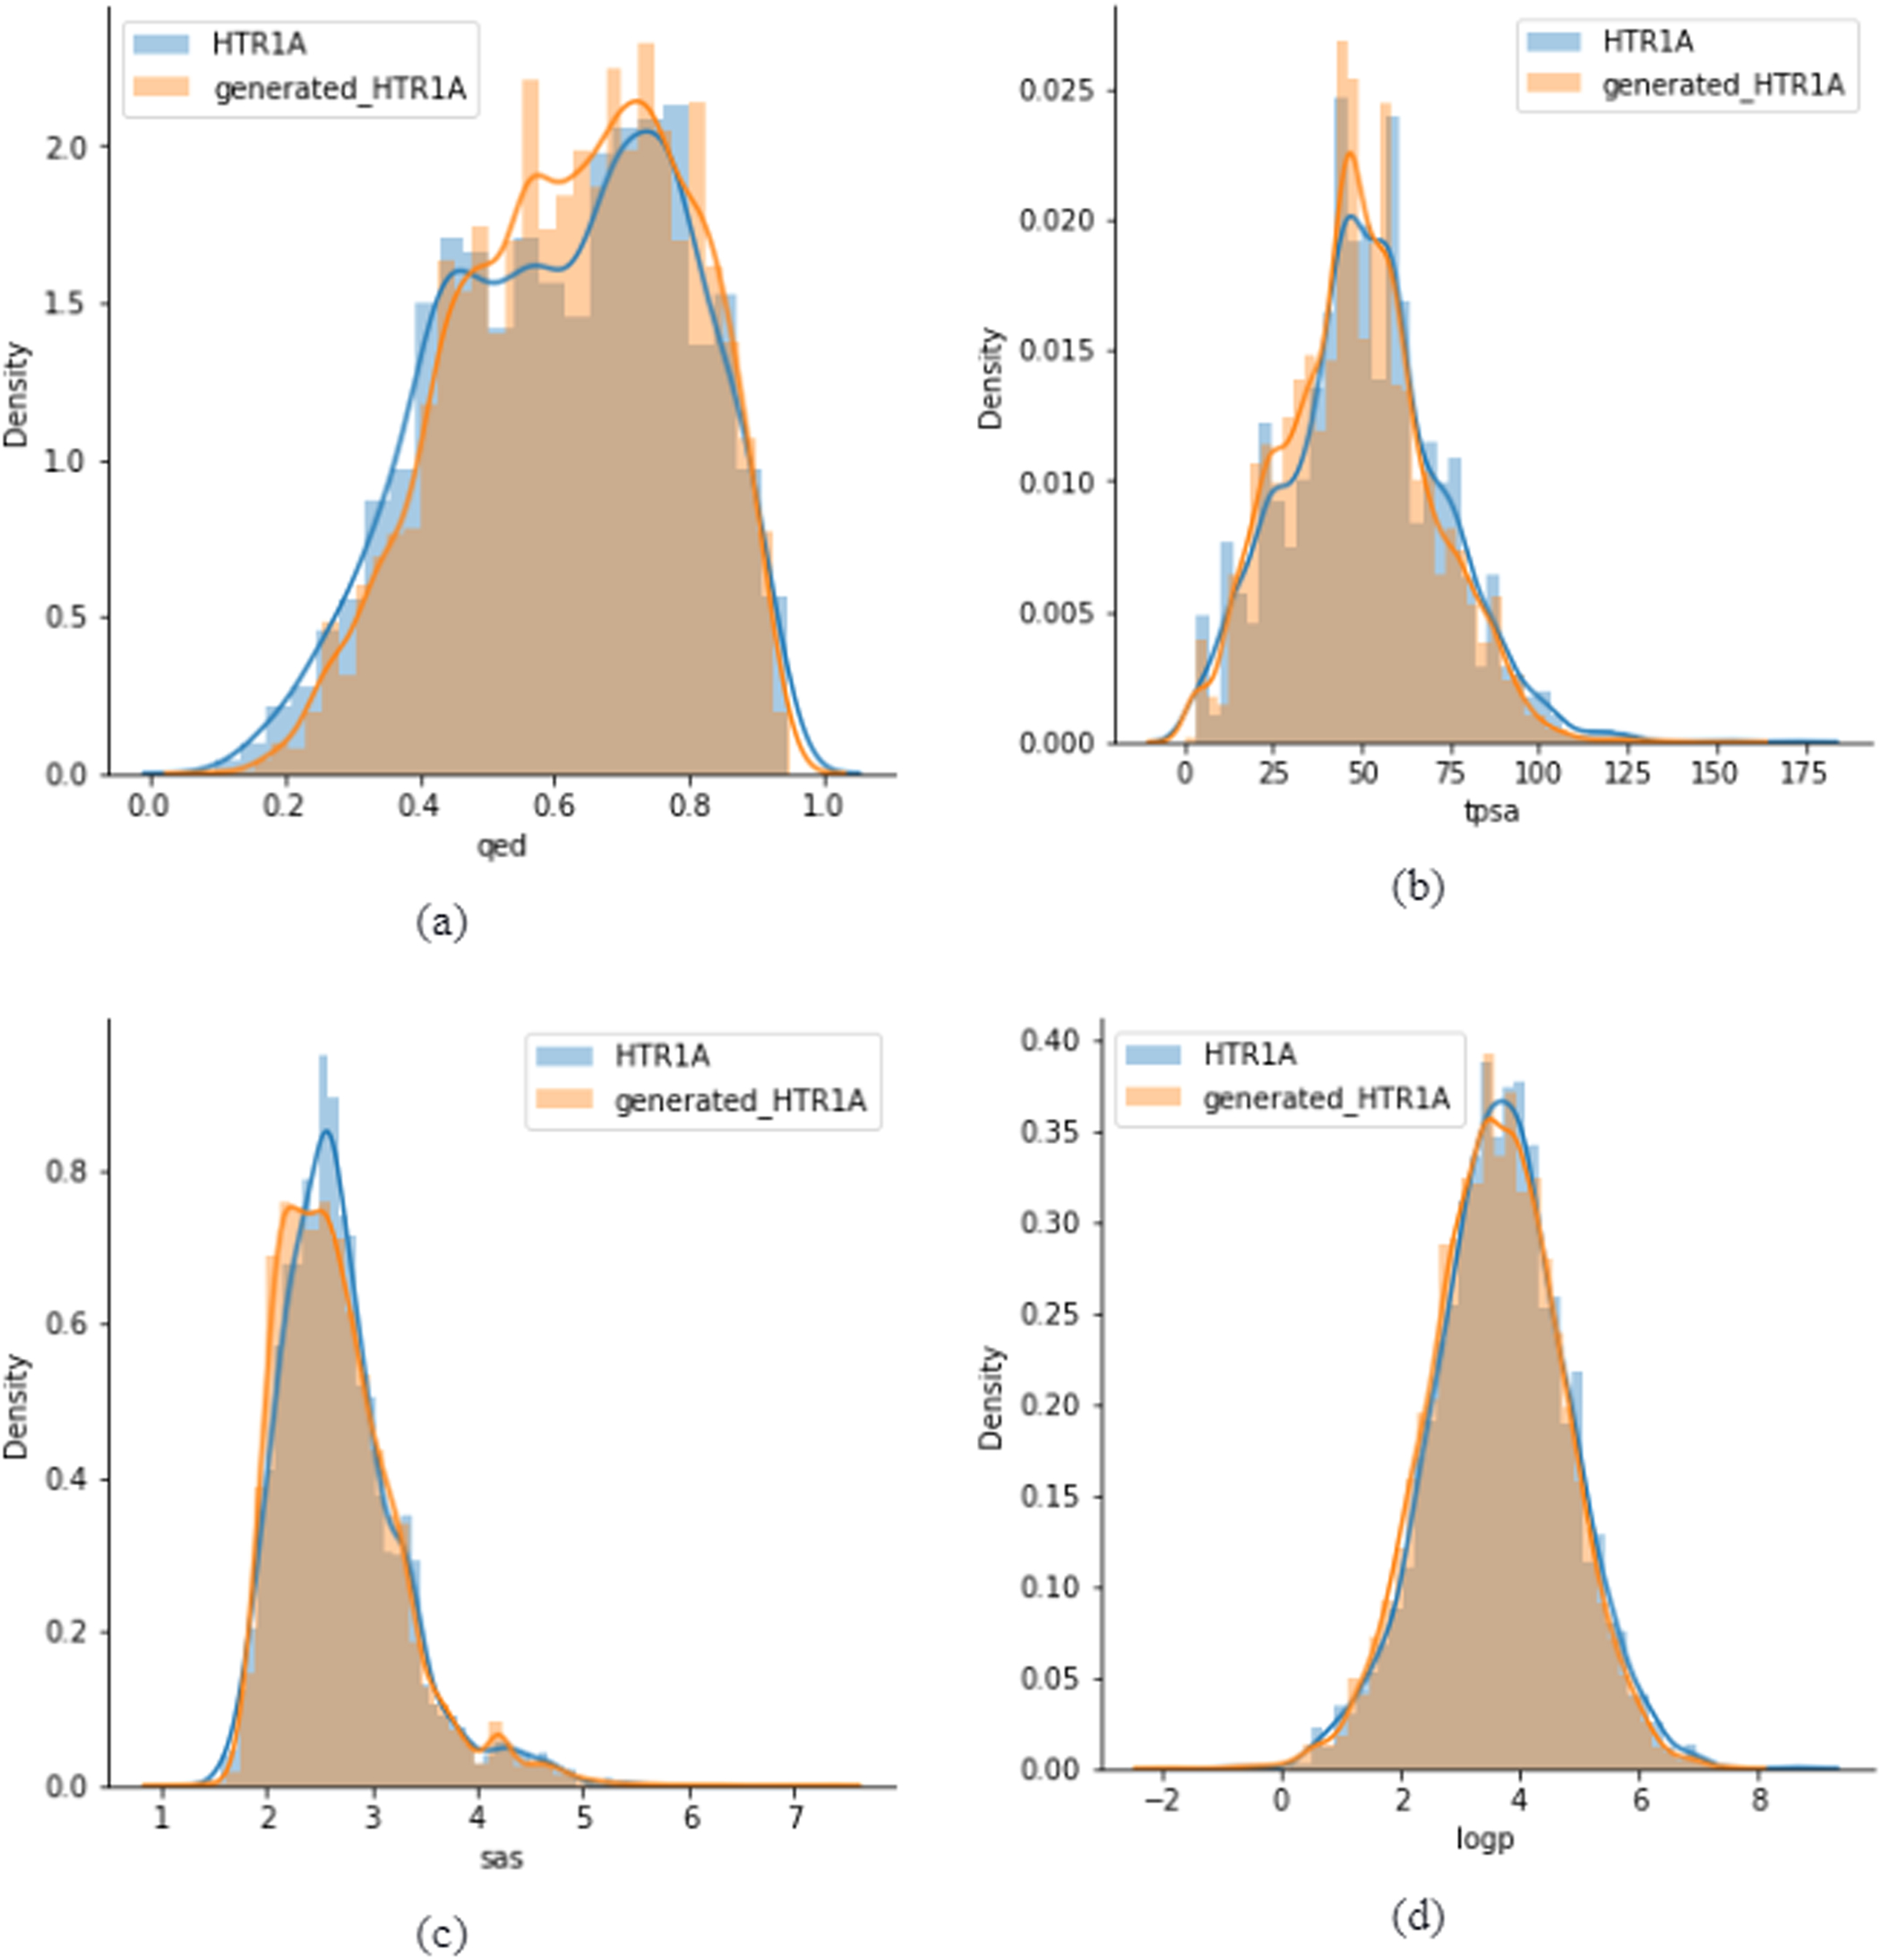
\includegraphics[width=\linewidth]{figures/8.png}
  \caption{采样的 HTR1A 中分子的特性(QED、TPSA、SAS 和 logP)分布以及相对关注生成的分子}
  \label{fig:8}
\end{figure}

表 \ref{tab:12} 报告了使用采样的 HTR1A 数据集相对关注条件生成的模型的性能。此外,图 \ref{fig:8} 可视化了采样的 HTR1A 数据集中分子的属性分布,以及使用相对注意力生成的分子。


图 \ref{fig:7} 和图 \ref{fig:8} 显示,即使数据集大小有限,具有相对注意力的模型也能够生成具有与训练集相似的属性分布的分子。

\begin{table}[H]
  \centering
  \caption{使用转移学习对 EGFR 非条件生成进行标准注意力和相对注意力训练的模型之间的比较}
  \label{tab:13}
  \begin{tabular}{llll}
    \hline 模型       & 有效性   & 唯一性   & 新颖性   \\
    \hline ModelGPT & 0.586 & 0.978 & 0.998 \\
    使用相对注意力的 MolGPT & 0.713 & 0.959 & 0.989 \\
    \hline
  \end{tabular}
\end{table}

表 \ref{tab:13} 提供了使用 EGFR 数据集进行非条件生成的标准注意力和相对注意力训练模型的性能比较。标准注意力模型生成了 58.6\% 的有效药物,而相对注意力模型在生成的 1000 个分子中获得了 71.3\% 的较高有效率。这表明有效性显着提高了 12.6\%。

\begin{table}[H]
  \centering
  \caption{使用转移学习对 EGFR 进行条件生成训练的模型的不同指标的比较}
  \label{tab:14}
  \begin{tabular}{llll}
    \hline 条件 & 有效性   & 唯一性   & 新颖性   \\
    logP      & 0.655 & 0.912 & 0.994 \\
    TPSA      & 0.757 & 0.841 & 0.993 \\
    SAS       & 0.717 & 0.854 & 0.985 \\
    QED       & 0.757 & 0.885 & 0.993 \\
    \hline
  \end{tabular}
\end{table}

表 \ref{tab:14} 显示了在 EGFR 数据集上训练相对注意力模型的性能,以使用迁移学习进行条件生成。

\begin{figure}[H]
  \centering
  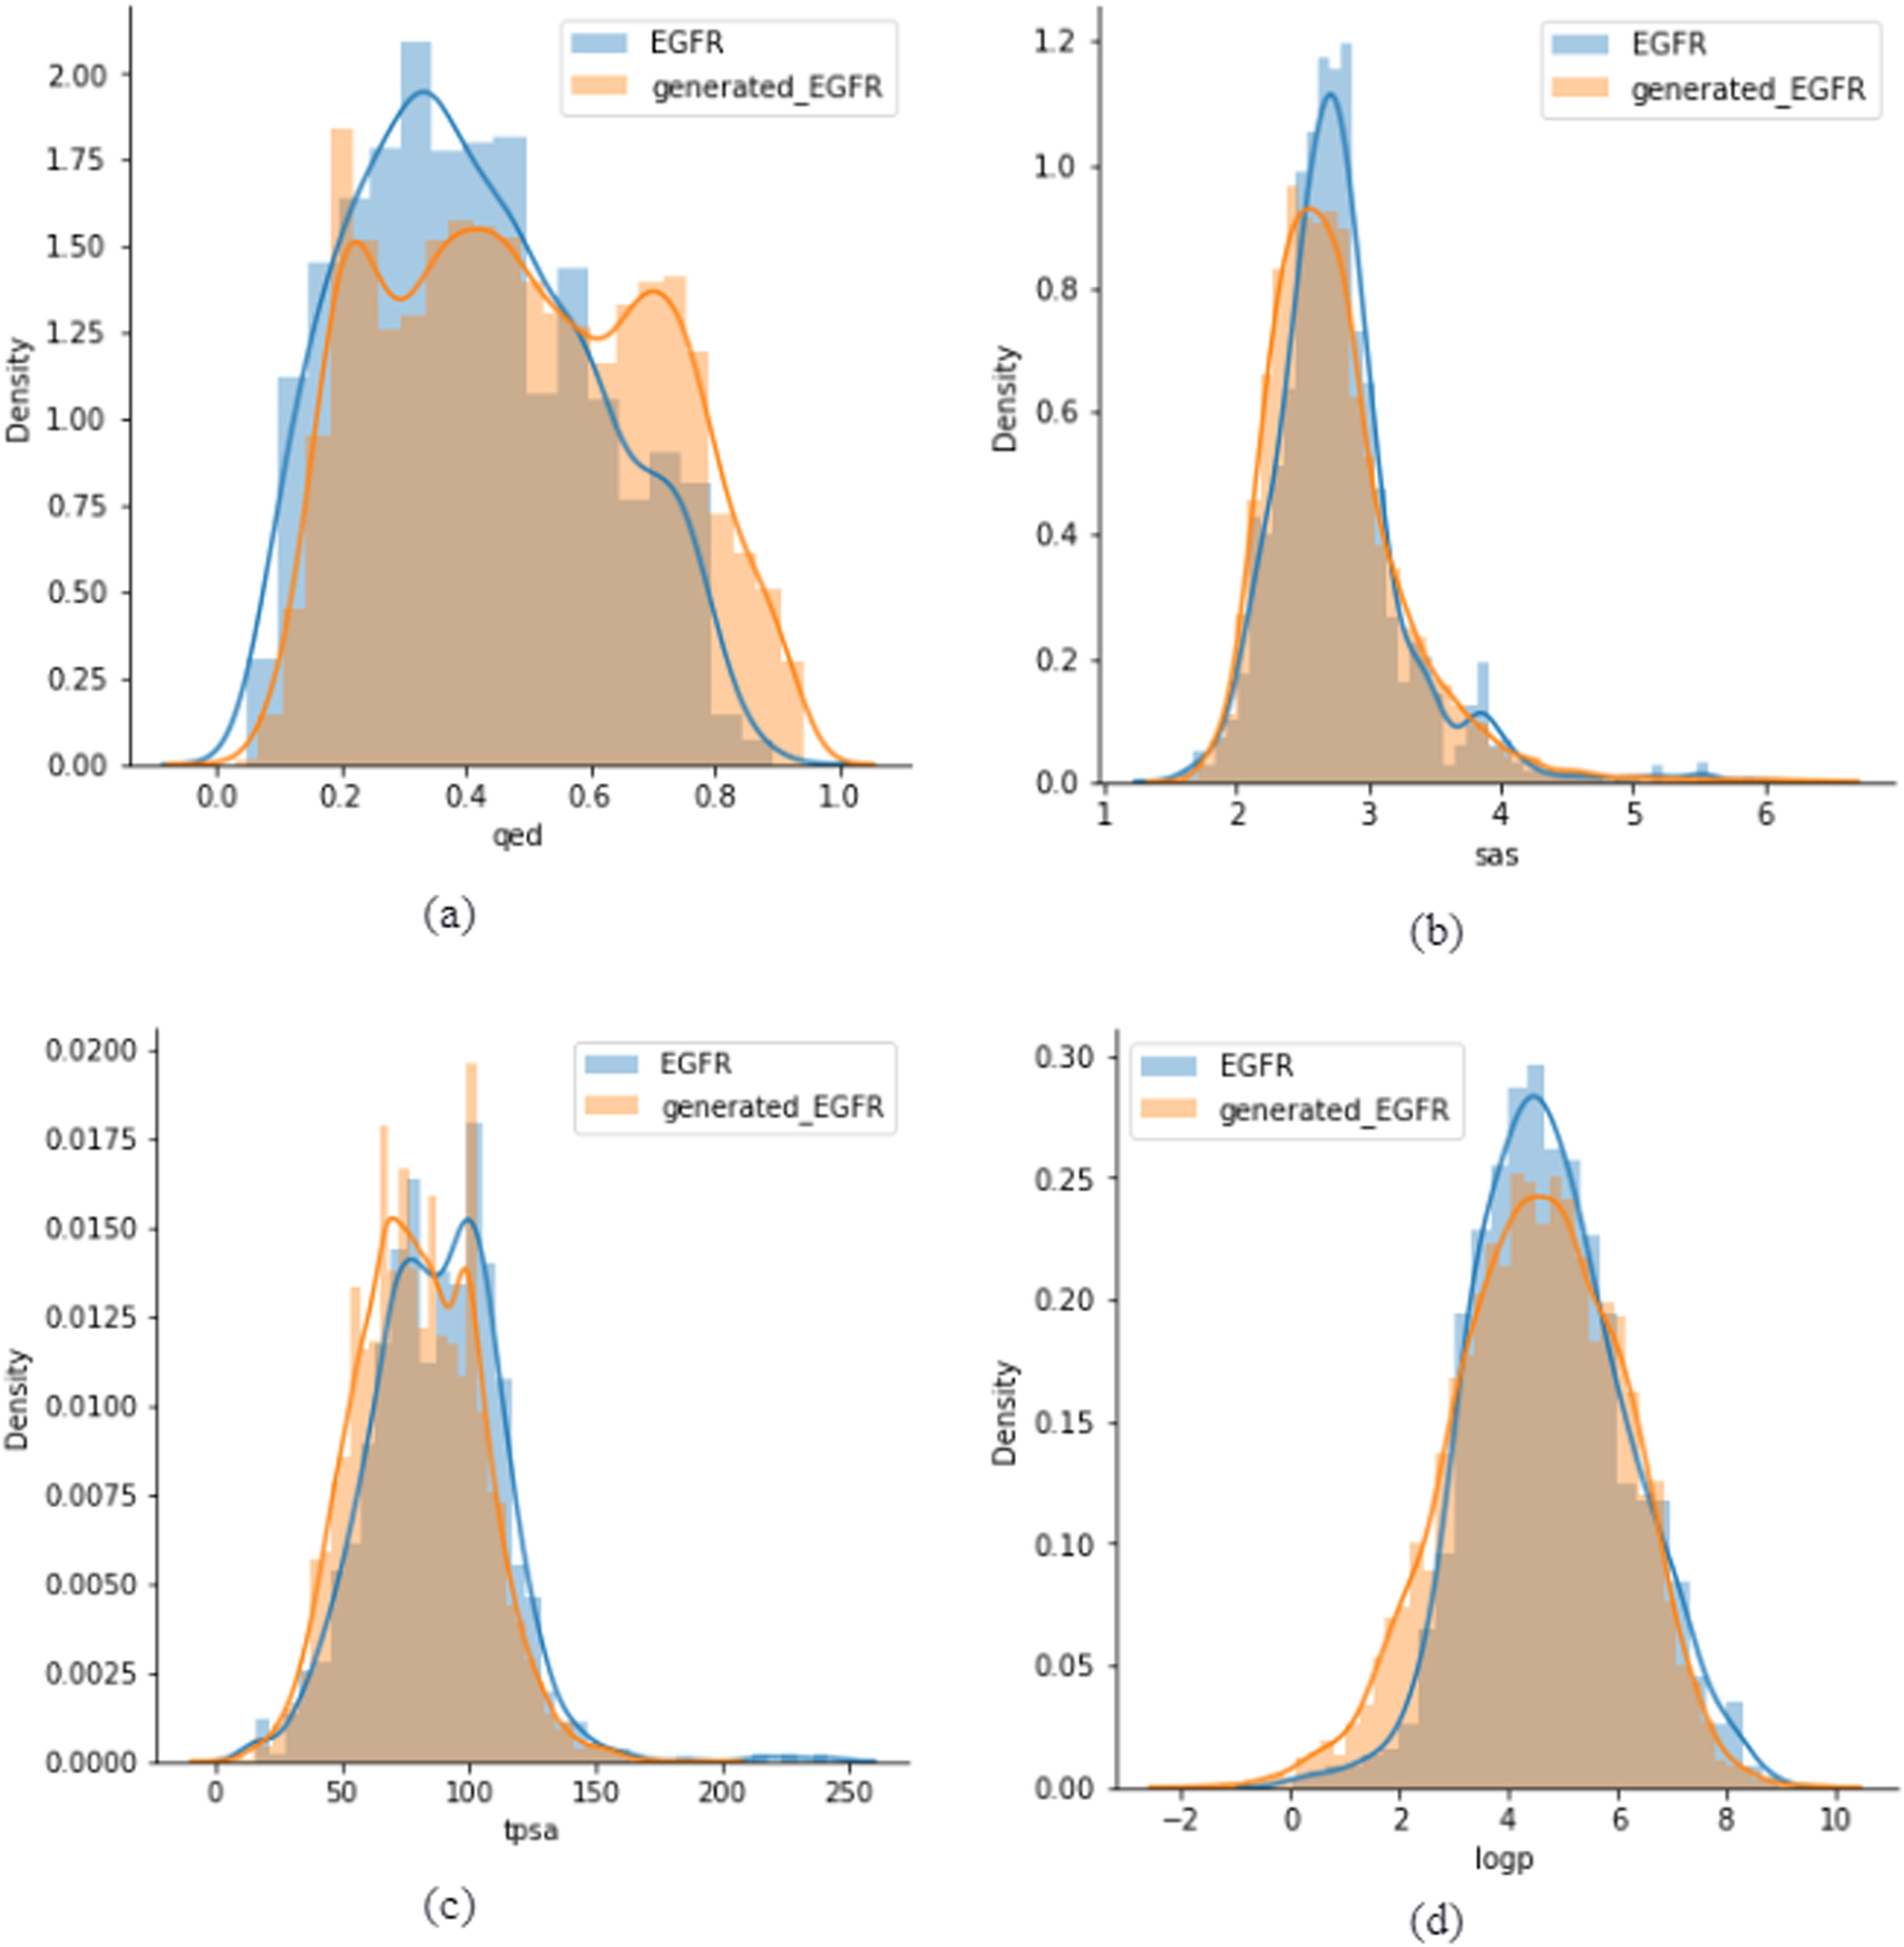
\includegraphics[width=\linewidth]{figures/9.png}
  \caption{EGFR 中分子的特性(QED、TPSA、SAS 和 logP)分布以及相对关注生成的分子}
  \label{fig:9}
\end{figure}

图 \ref{fig:9} 直观地表明生成的分子表现出与训练集相似的属性分布。

当使用 MOSES 数据集训练模型时,标准注意力的有效性为 99.4\%,而使用相对注意力时,有效性降至 99.2\%。同样,在 GuacaMol 数据集中,有效性从标准关注的 98.1\% 下降到相对关注的 97.8\%。当数据集足够大时,标准注意力足以学习 SMILES 所需的语法和语法。

然而,当应用于较小的特定目标数据集时,相对注意力的使用会带来更好的有效性。在表 9(采样的 S1PR1 数据集)中,有效性从 47\% 增加到 58.8\%。同样,在表 \ref{tab:11}(采样的 HTR1A 数据集)中,有效性从 85.2\% 提高到 86.3\%,在表 \ref{tab:13}(EGFR 数据集)中,有效性从 58.6\% 提高到 71.3\%。这些发现表明,当训练数据集大小有限时,利用相对注意力而不是标准注意力使模型能够更好地理解 SMILES 语法和化学规则。

当比较 GPT 模型与标准注意力和相对注意力在不同数据集上的性能时,当数据集足够大时,两种注意力机制都表现出相似的性能。然而,在使用迁移学习的小数据集进行特定目标药物设计的背景下,相对注意力比标准注意力有优势。

首先,它更好地捕获输入标记之间的依赖性,这在分子结构可以影响生物活性的药物设计中至关重要。通过考虑输入标记的相对位置,相对注意力可以准确地对它们的交互进行建模,从而改进预测。其次,相对注意力对于输入序列长度的变化更加稳健,这在处理训练样本有限的小数据集时很重要。

相比之下,标准注意力可能很难推广到不同长度的未见过的输入序列。 MolGPT 通过使用相对注意力来提高性能,特别是在小数据集上。这是因为它能够通过将相对位置信息纳入注意机制来更好地捕获序列中标记之间的关系。该模型生成了更多有效药物并更好地学习了数据统计。

通过应用迁移学习,该模型最初从更大的数据集(例如 MOSES)获取 SMILES 语法知识。随后,模型需要从更有限的数据集中适应和学习特定于目标特定药物的 SMILES 的语法。在这种情况下,相对关注被证明有利于促进学习的提高。它使模型能够快速掌握新的、未见过的标记的语法,这些标记可能存在于特定于目标的数据集中,但不存在于初始较大的数据集中。因此,与标准注意力相比,利用相对注意力的模型会生成更多数量的有效类药物分子,因为它能够从较小的数据集中更有效地学习这些新标记的语法。

\section{结论}

相对注意力是 Transformer 模型中使用的一种自注意力,已被证明可以增强需要标记相对位置的任务的性能,例如自然语言理解或图像字幕。它使模型能够捕获序列中不同位置之间的相互依赖性,而仅靠绝对位置编码和标准注意力可能无法捕获这些相互依赖性。

在这项研究中,我们利用变压器解码器模型中的相对关注来进行从头药物设计。我们的实验表明,具有相对关注度的 GPT 模型可以生成更有效、更独特、更新颖的药物,特别是当数据集很小且必须应用迁移学习时。模型中相对注意力的利用增强了 MOSES 数据集的新颖性,并提高了 GuacaMol 数据集的独特性。此外,我们证明了具有相对关注的模型可以学习和预测遵循训练集属性分布的分子。此外,该模型可以在条件生成过程中预测具有用户定义属性的分子。

当使用有限的数据集大小时,特别是在开发特定目标药物的背景下,使用相对注意力会显著提高模型性能。在评估具有相对关注的 MolGPT 模型在 MOSES 和 GuacaMol 数据集上的性能时,发现结果与具有标准关注的 MolGPT 所取得的结果相当。使用相对注意力的优势在这些数据集中并不那么明显,因为较大的数据集允许模型即使在标准注意力的情况下也能有效地学习 SMILES 语法。

通过利用 Huang 等人介绍的技术。为了计算相对位置编码,内存需求从 O(L$^2$D) 减少到 O(LD),其中 L 是序列长度,D 是隐藏状态维度。一个有前途的研究方向可能是使用相对位置编码和相对关注来学习目标蛋白质序列并生成具有改进的对接分数的分子。这将涉及将目标蛋白质序列作为模型的附加输入纳入其中。

应该指出的是,本研究中使用的模型仅仅是为了优化基本分子特性而设计的,并不能保证其在更复杂的任务(例如先导化合物优化)中的有效性。

\section{资金来源}

作者声明在手稿准备过程中没有收到任何赠款、资金或其他支持。

\section{作者贡献声明}

Suhail Haroon:概念化、方法论、软件、数据管理、写作 - 初稿。 Hafsath C.A.:写作 – 审阅和编辑、数据管理。 Jereesh A.S.:监督、项目管理。

\section{竞争利益声明}

无

\section{致谢}

无

\section{\textit{作者贡献}}

所有作者对这项工作做出了同等的贡献。所有作者阅读并认可终稿。

\printbibliography
\begin{translation-index}
\nocite{Haroon_C.a._A.s._2023}
\bibliographystyle{unsrtnat}
\printbibliography
\end{translation-index}
\end{translation}